\documentclass[12pt]{article}
%\topmargin=-0.5in
%\textheight=9in
%\evensidemargin=0in
%\oddsidemargin=0in
%\setlength{\textwidth}{6.5in}

\usepackage{algorithm}
\usepackage[noend]{algpseudocode}
\usepackage[autostyle]{csquotes}
\makeatletter
\def\BState{\State\hskip-\ALG@thistlm}
\makeatother

% Replace "Thesis Title", "Student name" etc. below with the correct values
% These values will then be automatically added wherever necessary in thesis-template.tex and defence-announcement.tex

\newcommand{\thesistitle}{Multilingual Digital Signage using Computer Vision and Bluetooth Beacons}
\newcommand{\studentname}{Suhas Dwarakanath}
\newcommand{\advisorname}{Dr. Brian Thoms}

% Custom commands for other often used strings (\pythonversion, \submissionyear etc.) can be added
% below using the following template
% \newcommand{\<commandname>}{<commandvalue>} 

\usepackage{amsmath,latexsym}
\usepackage{amsfonts}
\usepackage{amssymb}
\usepackage{amssymb}
\usepackage{graphicx}
%\usepackage{appendix}
%\usepackage{clrscode3e}
\usepackage{epstopdf}
\usepackage{subfigure}
%\usepackage{algorithm}
%\usepackage{algorithmic}
\usepackage{setspace}
\usepackage{color}
\usepackage{listings}
\usepackage{setspace}
\usepackage{algpseudocode}
\usepackage{algorithm}
\usepackage[all]{xy}
\usepackage{pdfpages}
\usepackage{titlesec}

% Ensures a new section is on its own page. Must be done before hyperref is loaded

%changed by Suhas

 \newcommand{\sectionbreak}{\clearpage}

% Clickable references
\usepackage[hidelinks]{hyperref}

% Ensures graphic is in view after clicking on a reference to see it
\usepackage[all]{hypcap} 


% \doublespacing
\renewcommand{\topfraction}{0.9}	% max fraction of floats at top
\renewcommand{\bottomfraction}{0.8}	% max fraction of floats at bottom

%   Parameters for TEXT pages (not float pages):
\setcounter{topnumber}{2}
\setcounter{bottomnumber}{2}
\setcounter{totalnumber}{4}      % 2 may work better
\setcounter{dbltopnumber}{2}    % for 2-column pages
\renewcommand{\dbltopfraction}{0.9}	% fit big float above 2-col. text
\renewcommand{\textfraction}{0.07}	% allow minimal text w. figs

%   Parameters for FLOAT pages (not text pages):
\renewcommand{\floatpagefraction}{0.7}	% require fuller float pages
    
% N.B.: floatpagefraction MUST be less than topfraction !!
\renewcommand{\dblfloatpagefraction}{0.7}	% require fuller float pages

\newenvironment{dig}{\\ [6pt]\noindent {\bf Digression}}{~$\Box$\\ [6pt]\indent}
\newenvironment{dig1}{\noindent {\bf Digression}}{~$\Box$\\ [6pt]\indent}
\newtheorem{alg}{\hspace{1.3in} Algorithm}
\newtheorem{thrm}{Theorem}
\newtheorem{lemm}[thrm]{Lemma}
\newtheorem{conj}[thrm]{Conjecture}
%\newtheorem{claim}[thrm]{Claim}
\newtheorem{prop}[thrm]{Proposition}
\newtheorem{defn}[thrm]{Definition}
\newtheorem{obs}[thrm]{Observation}

\hyphenation{Chris-to-dou-lak-is}
\def\proof{\bigbreak\noindent {\sl Proof.\/}\enspace}
\def\qedbox#1#2{\vbox{\hrule height.2pt
  \hbox{\vrule width.2pt height#2pt \kern#1pt \vrule width.2pt}
  \hrule height.2pt}}
\def\qed{\hfill \quad\qedbox46\newline\smallbreak}

\def\s#1{\mbox{\boldmath $#1$}}
\def\floor#1{\lfloor #1 \rfloor}
\def\bfloor#1{\big\lfloor #1 \big\rfloor}
\def\Bfloor#1{\Big\lfloor #1 \Big\rfloor}
\def\ceil#1{\lceil #1 \rceil}
\def\bceil#1{\big\lceil #1 \big\rceil}
\def\+{\!+\!}
\def\-{\!-\!}
\def\plmi{\!\pm\!}
\def\m{\!-\!}
\def\uu#1{\underline{#1}}
\def\o#1{\overline{#1}}
\def\itbf#1{\textit{\textbf{#1}}}
\def\match{\approx}
\def\cP{\mathcal{P}}
\def\G{\mathcal{G}}
\def\B{\mathcal{B}}
\def\O{\mathcal{O}}

\def\bproc{{\bf procedure\ }}
\def\bfunc{{\bf function\ }}
\def\bvar{{\bf var\ }}
\def\barray{{\bf array\ }}
\def\bof{{\bf of\ }}
\def\bfor{{\bf for\ }}
\def\bnull{{\bf null\ }}
\def\bto{{\bf to\ }}
\def\bdownto{{\bf downto\ }}
\def\bwhile{{\bf while\ }}
\def\brep{{\bf repeat\ }}
\def\buntil{{\bf until\ }}
\def\band{{\bf and\ }}
\def\bor{{\bf or\ }}
\def\bdo{{\bf do\ }}
\def\bif{{\bf if\ }}
\def\bthen{{\bf then\ }}
\def\belse{{\bf else\ }}
\def\belsif{{\bf elsif\ }}
\def\bnot{{\bf not\ }}
\def\bgoto{{\bf goto\ }}
\def\bcontinue{{\bf continue\ }}
\def\breturn{{\bf return\ }}
\def\bbreak{{\bf break\ }}
\def\boutput{{\bf output}}
\def\la{\leftarrow}
\def\ra{\rightarrow}
\def\llra{\Leftrightarrow}
\def\q{\quad}
\def\qq{\qquad}
\def\com#1{{\bf $\triangleright$}\hspace{6pt}{\sl #1}}
\def\rem#1{\hspace{24pt}{\sl #1}}
\def\pref(#1,#2){$#1$ is a prefix of $#2$}
\def\suff(#1,#2){$#1$ is a suffix of $#2$}
\def\FIND{\mbox{FIND}}
\def\reg(#1,#2){$#2$ is $#1$-regular}
\def\notreg(#1,#2){$#2$ is not $#1$-regular}
\def\top{\tt{top}}
\def\pop{\tt{pop}}
\def\push{\tt{push}}
\def\true{\tt{true}}
\def\false{\tt{false}}
\def\UPDATE\_F{\tt{UPDATE\_F}}
\def\LEAST{\tt{LEAST}}
\def\MERGE{\tt{MERGE}}
\def\mec{\tt{mec}}
\def\MEC{\tt{MEC}}
\def\CMEC{\tt{CMEC}}
\def\MELC{\tt{MELC}}
\def\CMELC{\tt{CMELC}}
\def\MELS{\tt{MELS}}
\def\CMELS{\tt{CMELS}}
\def\MCNT{\tt{MaxCount}}
\def\CLEN{\tt{CorLen}}

% \def\B{\tt{B}}
\def\Q'{\tt{Q'}}
\def\CP{\tt{CP}}
\def\MNC{\tt{MNC}}
\def\PR{\tt{PR}}
\def\PRS{\tt{PRS}}
\def\CPR{\tt{CPR}}
% \def\POS{\tt{POS}}
\def\LEN{\tt{LEN}}
\newcommand{\dd}{\mathinner{\ldotp\ldotp}}

\newif\ifShow
\Showfalse
% MATH -----------------------------------------------------------
\newcommand{\norm}[1]{\left\Vert#1\right\Vert}
\newcommand{\abs}[1]{\left\vert#1\right\vert}
\newcommand{\set}[1]{\left\{#1\right\}}
\newcommand{\Real}{\mathbb R}
\newcommand{\eps}{\varepsilon}
\newcommand{\To}{\longrightarrow}
\newcommand{\BX}{\mathbf{B}(X)}
\newcommand{\A}{\mathcal{A}}
% Algorithm ------------------------------------------------------

\algnewcommand{\LineComment}[1]{\State \(\triangleright\) \normalfont{\sl #1}}
\algtext*{EndWhile}% l
\algtext*{EndIf}% Remove "end if" text
\algtext*{EndFor}% Remove "end for" text
\algtext*{EndFor}% Remove "end for" text
\algtext*{EndProcedure}% Remove "end procedure" text

% manifold
\newcommand{\F}{{F}}
\newcommand{\scF}{\F}
\newcommand{\X}{{X}}
\newcommand{\Fhat}{\widehat\F}
\newcommand{\scN}{{\EuScript N}}
\newcommand{\scL}{{\EuScript L}}
\newcommand{\PP}{\mathbb P}
\newcommand{\R}{\mathbb R}
\newcommand{\C}{\mathbb C}
% \newcommand{\CP}{\C\PP}
\newcommand{\CH}{\C{\mathrm H}}
\newcommand{\Lie}{{\mathcal L}}
\newcommand{\cpn} {\CP^n}
\newcommand{\chn} {\CH^n}
\newcommand{\cptwo} {\CP^2}
\newcommand{\chtwo} {\CH^2}
\newcommand{\chone} {\CH^1}
%\newcommand{\mean}{{\mathcal m}}
\newcommand{\mean}{{\mathbf m}}
%\def\({\left (}
\def\({\left(}
%\def\){\right )}
\def\){\right)}
\def\<{\langle}
\def\>{\rangle}
\def\a {\alpha}
\def\b {\beta}
\def\l {\lambda}

% Pfaffian systems
\newcommand{\CC}{{\EuScript C}}
\newcommand{\I}{{\mathcal I}}
\newcommand{\J}{{\EuScript J}}
\newcommand{\K}{{\mathcal K}}
\newcommand{\Khat}{\widehat{\K}}
\newcommand{\M}{{\mathcal M}}
\newcommand{\V}{\mathcal V}
\newcommand{\calS}{\mathcal S}

% differential forms
\newcommand{\w}{\omega}
\newcommand{\kh}{\hat\kappa}
\newcommand{\diff}{{\operatorname{diff}}}
% \newcommand{\alg}{{\operatorname{alg}}}

%maps
\newcommand{\fhat}{\hat{f}}

%open sets
\newcommand{\setU}{\EuScript U}
\newcommand{\Uhat}{\widehat{\setU}}

% vectors
\newcommand{\e}{\mathbf e}
\newcommand{\ehat}{\hat{\e}}
\newcommand{\bv}{\mathbf v}
\newcommand{\bx}{\mathbf x}
\newcommand{\bg}{\mathbf g}
\newcommand{\by}{\mathbf y}
\newcommand{\bw}{\mathbf w}
\newcommand{\bxi}{\mathbf\xi}
\newcommand{\bn}{\mathbf n}
\newcommand{\bz}{\mathbf z}

% complex variables
\newcommand{\ri}{\mathrm i}
\newcommand{\realpart}{\operatorname{Re}}

% operators
\newcommand{\JJ}{{\mathrm J}} % complex structure
\newcommand{\RR}{{\sf R}} % curvature operator
\newcommand{\Ric}{{\sf Ric}} % Ricci tensor
\newcommand{\di}{\partial}
\newcommand{\dib}[1]{\di_{#1}}
\newcommand{\tvec}{\tfrac{\di}{\di t}}
\newcommand{\restr}{\negthickspace \mid}
\newcommand{\transpose}[1]{{}^t\hskip-2pt{#1}}
\newcommand{\nat}{\widetilde\nabla}
\newcommand{\RRt}{\widetilde R}
\newcommand{\mt}{\widetilde M}
\def\intprod{\mathbin{\raisebox{.4ex}{\hbox{\vrule height .5pt width
5pt depth 0pt %
         \vrule height 3pt width .5pt depth 0pt}}}}
\newcommand{\hook}{\intprod}
\def\&{\wedge}
% \def\s{\sigma}
\def\a{\alpha}
\def\b{\beta}
\def\n{\nabla}

\title{\thesistitle} 
\author{\studentname}
\date{\today}

\begin{document}

\begin{titlepage}
\pagenumbering{gobble}
\begin{center}
{\Large \bfseries \thesistitle \par}

\vspace{2 cm}
\baselineskip = 2\baselineskip
A Thesis Presented to \\
The Faculty of the Computer Science Department\\
California State University Channel Islands

\vspace{1 cm}

In (Partial) Fulfillment\\
of the Requirements for the Degree\\
Masters of Science in Computer Science\\

\vspace{1 cm }

\vfill

by \\
\studentname\\
Advisor: \advisorname\\
March 2019
\end{center}
\end{titlepage}
\baselineskip = \baselineskip
\newpage

\null
\vfill
\begin{flushleft}
\copyright\; 2019\\
\studentname\\
ALL RIGHTS RESERVED
\end{flushleft}
\newpage

\begin{center}
{\large \bfseries APPROVED FOR MS IN COMPUTER SCIENCE \par}

\vspace{1.5 cm}

\hrulefill\\
{\large \bfseries Advisor: \advisorname \hfill Date \par}

\vspace{1.5 cm}

\hrulefill\\
{\large \bfseries Name \hfill Date \par}

\vspace{1.5 cm}

\hrulefill\\
{\large \bfseries Name \hfill Date \par}

\vspace{3 cm}

{\large \bfseries APPROVED FOR THE UNIVERITY \par}

\vspace{1.5 cm}

\hrulefill\\
{\large \bfseries Name \hfill Date \par}
\end{center}
\newpage

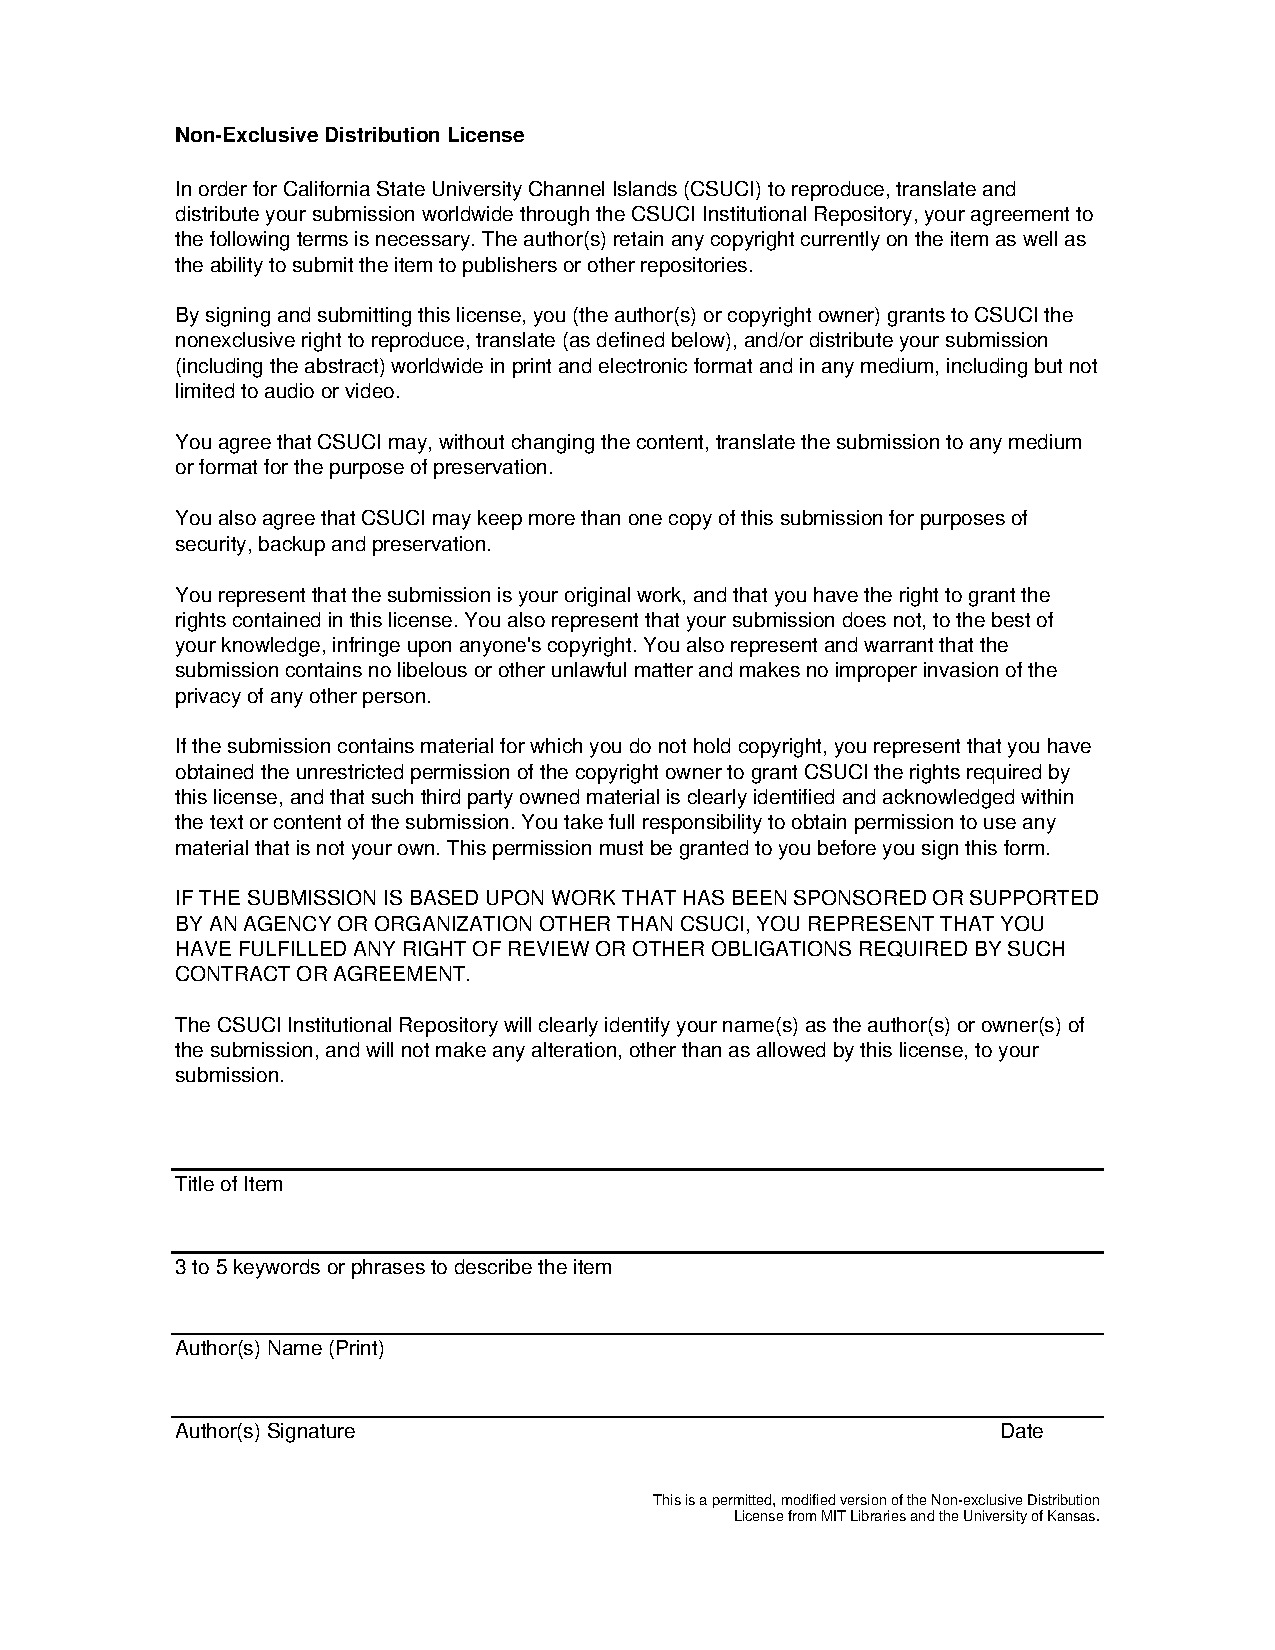
\includepdf{media/distribution-license.pdf}
\newpage


\maketitle

\begin{abstract}
Due to rapid globalization and changing lifestyle, more people are now visiting foreign countries for business and travel. However, important signages like traffic signs, safety signs and informational signs are displayed in only one language (usually the native language). There are many languages in the world and it is impractical to install signages in all the languages. In this research, by combining computer vision and bluetooth beacons, multilingual digital information is displayed on the user's smartphone. A mobile application is constructed which enables the user's smartphone to listen to nearby digital signages (with bluetooth beacons) and display the respective signage information in user's preferred language. The application also enables the user to capture an image of a printed signage, extract the information in the signage and translate the information to user's preferred language. Optical Character Recognition (OCR) is used to extract the text from the image and Google Translate is used for the language translation. This system was implemented in the university campus and experiments were conducted by to determine the feasibility of using this system on a larger scale. It was found that the system helps the users to understand their surroundings better in their preferred language.
\end{abstract}

\newpage
\pagenumbering{roman}

\tableofcontents

\newpage

\listoffigures
\listoftables

\newpage
\pagenumbering{arabic}

\section{Introduction}
\label{sect-intro}

With changing lifestyle and globalization, more people visit foreign countries. Every country is working towards becoming tourism oriented to increase their economy. Most of the visitors use their smartphone to access information \cite{audioBeacon}. However, when visiting foreign countries, most people face difficulties in obtaining information due to difference in language, which makes it an inconvenience to stay in foreign countries for a longer time. \cite{one}. Recently, a lot of refugee and migrant families from all over the world faced a lot of struggles at the U.S immigrations. A lot of these refugees faced problems with the documentation because they could not understand the content of the legal documents. It is natural for people to understand information better in their home language. Therefore, an effective method of providing and accessing information in multiple languages is required. \\

In this study, in order to solve such problems, a multilingual information service is developed using Computer Vision and Bluetooth beacons. The information can be accessed from the user's smartphone in most of the major languages. We focus on the smartphone's camera to 'see' information in multiple languages. We also use bluetooth beacons to 'push' information to smartphones in proximity. The user can then access the information in multiple languages. By using this method, we expect people visiting foreign countries to access information naturally in the same way they would in their home countries. This paper evaluates various options like GPS, NFC and RFID which could be used to provide information based on user's location. We then describe the required functions and configuration of the prototype system developed. \\

\subsection{Motivation}
\label{motive}
\paragraph{}When visiting foreign countries, it is essential to understand critical information around you. When visiting points of interest in a foreign land, many visitors would like to learn more about the place - the history, significance of the place and other critical information. In many cases, this information is displayed on signages, usually in the local language of the country. 

\paragraph{} In recent years, refugee families arriving in the United States of America are required to deal with a lot of new information including legal documents and signs. Many refugees would not be well versed with English and thus, there is a need for a system which can extract text from the documents and translate it to a language which the individual can understand. 

\paragraph{}This study is inspired by the above problems people are facing right now and aims to provide a low cost solution using computer vision and bluetooth iBeacon technologies.

%An example reference: \autoref{fig:ci-logo} (Notice references and citations are clickable!)

% When including grapics, make sure the directory is relative to root .tex document, not the current .tex file

%\begin{figure}[H]
%	\centering
%	
\includegraphics[width=0.7\linewidth]{media/ci-logo}
%	\caption{This is an example graphic}
%	\label{fig:ci-logo}
%\end{figure} 

\section{Background}
\label{sect-background}

\paragraph{}Text extraction and text translation are highly researched areas in the field of computer vision to model a smart self-learning system, which include text associated with banners, highway and roadside sign boards or the information on local transport system. This information in the form of text provide significant clues about that environment \cite{india}. Text detection can also help those who are visually impaired and tourist alike to convey the right information in more understandable way \cite{india}.

\paragraph{}As a method of accessing information on public signages, there are two ways of using a smart phone to find information in relevant languages; the user needs to search information by himself or herself, then translate it relevant language to access necessary information. Alternatively, when digital signage is used, the user can find and access information by coming in proximity of the digital signage without performing any special action. In this study, we explore ways to improve searching and accessing information by using smartphone camera and the method of information provision using the digital signage using iBeacons. This should make users who visit foreign countries get information without making extra efforts. 

\subsection{Related Work}

\paragraph{} A study of multilingual digital signage using iBeacon communication was done, for the purpose of evaluating the technology in an university campus at Japan \cite{one}.  In the experiment, the authors installed 25 iBeacon devices at sightseeing spots, restaurants, souvenir shops, photo shops, etc. in Shirakawa-go, a popular tourist area of Japan. When visitors look at these heritage spots, it is difficult for them to understand whether it is a restaurant or a souvenir shop. By using this system, tourists were able to obtain necessary information in their native languages when they enter each iBeacon area while walking in Shirakawa-go. The paper confirmed that this system can be used effectively for both Japanese and the foreigners \cite{one}.  In their system, it was possible to change the displayed language automatically when the user comes near to the digital signage, by using the mechanism of background scanning of iBeacons. However, their study is dependent on installing and configuring bluetooth iBeacons for the user to be able to understand the signages. It does not support text translations from printed signages. In our study, we aim to support both digital and printed signages.

\paragraph{}American MLB has been using iBeacons in some stadiums. Their mobile application can provide navigation system, so the ticket in user's hand will pop out automatically and their position will be tracked when they get close to ticket entrance. Many techniques such as the method of displaying information written in several languages in user's native language, the method of displaying multilingual information simultaneously, and the method of switching displayed language using touch screens, have been used. \cite{zoo} When iBeacon is scanned by the nearest mobile application, the proximity of the beacon will be accessed and customers will be provided with service based on the proximity \cite{taiwan} \cite{room}.

\paragraph{}In India, a study of text detection and extraction based on Stroke Width Transform (SWT) to extract letters was conducted \cite{india}. This application focussed on tourism industry and local transport, to help people to deal with different languages in India which involve text associated with natural scenes in the local public places. Using SWT method, various Indian languages and their combination with English were detected. However, this study only translates the regional languages used in India and does not translate the detected texts into International languages languages. This is still a hindrance for foreigners to understand their environment.

\paragraph{} To develop a location-based system such as the digital signage system in our study, accurately determining user's proximity to the signage is important. The problem of proximity detection is found to be difficult in a variety of environments. Existing approaches like Global Positioning System and Wi-Fi triangulations are insufficient to meet the requirements of high accuracy and also involve high cost to setup. A study was made using, Bluetooth which is commonly available in all smartphones to find the proximity over shorter distance and determine the distance based on the Received Signal Strength Indicator (RSSI) values of the Bluetooth  beacons \cite{distance}. In existing systems, GPS is used to find the location, which won't work as accurately indoors and inside most commercial building areas. So the authors proposed a system to overcome the problem by using Bluetooth to Bluetooth proximity estimation. By using the received signal strength of the Bluetooth device, RSSI value is used to find out the approximate distance between the devices. This technique helps in determining the location of nearby user. The study proposed the proximity determination model by combining Bluetooth RSSI value. The results demonstrate that Bluetooth offers a feasible mechanism that is accurate and power-efficient for measuring user's proximity indoors \cite{distance}. While this study does not focus on text detection or digital signage, this is  useful for our study to determine the distance of the user/smartphone to the iBeacons.

\paragraph{}Optical Character Recognition (OCR) is the electronic conversion of images into machine encoded text. It provides alpha-numeric recognition of printed and handwritten characters. In the recent past, OCR has been an active topic of research and has wide applications in healthcare, banking, finance and education. One of the applications of OCR is to help with visually impaired persons. According to the World Health Organization (WHO), around 285 million people around the world are estimated to be visually impaired, out of which 90\% live in developing countries. Thus there is a definite need to develop a system to provide information to the visually impaired. In the research by S. Sonth and J. S. Kallimani, a camera based framework was built on the Raspberry Pi, integrating with Image processing algorithms, OCR and Text-to-Speech (TTS) module \cite{ocr}. The smartphone camera is used to capture an image of the printed or handwritten text, and the image was then subject to preprocessing before being fed into the OCR system \cite{ocr}. This study, however does not focus on language translation or digital signage, we adopt image pre-processing techniques like binarization, de-noising, de-skewing, segmentation and feature extraction in our research.

\paragraph{}In Taiwan, to encourage learning English, a study was carried out using the iBeacon's micro-positioning function to set the location in museum, restaurant, store, etc. When user's mobile phone detects the presence of iBeacons, the mobile application facilitates learning by interacting with users' environment \cite{taiwan}. Vocabulary includes the single words and expressions commonly used in daily life. With the narration and use of everyday sentence structure and grammar, users can learn English conveniently and quickly and apply it to real situations. In this way, users can learn English from the surroundings to enhance their English ability, achieve better effects with minimal efforts and in a fun way in the proposed system. With the combination of the proposed application, English learning materials and iBeacon micro-location feature, learners can receive the surrounding related learning materials. In this manner, learners will have chance to build the connection between the learning materials and the environment which can enforce their memory to remember the learning concept \cite{taiwan}. It was found that the system can raise the learning intent of the learners and may improve their learning effectiveness. However, this study focusses on converting Chinese language to English based on the user's location. It does not support multiple languages and the system is entirely dependent on iBeacons.

\paragraph{} With the rapid rise in multimedia and data services, demand for positioning has increased, especially in indoor environment which needs to determine the proximity  of the user to provide context based information \cite{services}. There is a lack of accuracy in current positioning systems. A study was made to design and develop a mobile-based indoor location system for mobile applications with the Bluetooth Low Energy technology based on the iBeacon \cite{indoor}. The authors adopted Gaussian filter and Unscented Kalman filter method to read signals from iBeacon device. With the extracted signals, the authors compared them with a database. They were able to display data based on micro-location on the user's smartphone.  It was found that the iBeacon approach has better performance compared with WiFi method  \cite{indoor}. However, this study does not translate the detected texts into the user's preferred languages. This is still a hindrance for foreigners to understand their environment.

\subsection{Outline}

\paragraph{}With the recent developments in Internet of Things (IoT), the user and their location is closely interrelated. The outdoor positioning system based on satellite position (GPS) has been getting more accurate. However, GPS positioning satellite signals can only be best used in outdoor environments, it is difficult to meet the needs of indoor positioning  \cite{indoor}. So, there is an urgent demand for indoor positioning technology and providing micro-location-aware data. Micro-location is a term used to define the location, accurate down to a few meters. 

\paragraph{}In recent years, many types of short-range wireless communication protocol and related products are emerging in the market. Some of the short-range wireless data communication includes WIFI, Bluetooth, ZigBee, RFID, NFC and Ultra Wideband (UWB) among other types of technology \cite{indoorPositioning}. These technologies play an important role in their respective areas and requirements. Let us evaluate some of the options we have to provide data based on micro-location.

\subsubsection{GPS}
\paragraph{} The outdoor positioning system, which is based on global satellite position (GPS) provides users with the needs of positioning, accurate to 10 meters. However, GPS positioning satellite signals is only feasible in outdoor environment. GPS fails to determine the user's location accurately inside a building or within a room \cite{indoor}. This means, we cannot use GPS in our study as we need to determine users location, with accuracy ranging from 0.1 to 50 meters.

\subsubsection{Wi-Fi}
\paragraph{} The coverage of Wi-Fi is wide. It could reach 100 meters, and achieve coverage with comprehensive in clear surroundings. Also, the speed of network transmission is higher, it’s useful for real-time interaction of the application. The Wi-Fi network construction has a low cost, is easy to maintain and very suitable for use in mobile phones. However, the core drawbacks are that data security and performance are slightly less compared to Bluetooth \cite{indoor}. It is also difficult to accurately triangulate the user's position inside the network.

\subsubsection{Near Field Communication (NFC)}
\paragraph{}NFC is a set of short-range wireless technologies that enable two electronic devices, one of which is usually a smartphone, to establish communication by bringing them in close proximity. However, the range  of NFC is less than 10 centimeters and it gets very expensive to install a lot of NFC tags to achieve the required proximity services \cite{tracking}. Thus, it is not feasible to use NFC in our study.

\subsubsection{Bluetooth}
\paragraph{}Bluetooth is a radio technology which supports short distance communication. The main advantage of Bluetooth indoor positioning technology is that, Bluetooth chips are small, easy to integrate with mobile phones and even in smaller devices. On the other hand, the shortcomings of Bluetooth technology are;  relatively high power consumption and lack of stability when the system is setup in complex space environment \cite{indoor}. 

\subsubsection{iBeacon}
\paragraph{}The communication protocol used in iBeacon is the Bluetooth Low Energy (BLE). Bluetooth version 4.0 devices supports BLE \cite{indoor}. iBeacon communication frequency works on the 2.4GHz band, which is as fast as the Wi-Fi. iBeacon has proximity sensing technology, it can transfer information such as Uniform Code of unique ID (UUID). Mobile applications can scan and read the information about UUID and RSSI, and it can be transformed into a physical location, which triggers location-aware applications and information. iBeacons are also low-cost devices and typically run for a year on a single coin battery such as CR2032 \cite{audioBeacon}. This makes it feasible for us to implement iBeacons into out study of providing data based on user's micro-location.

\subsubsection{Comparison of indoor positioning methods}
\paragraph{} The table below presents the advantages and disadvantages of various indoor positioning systems \cite{sensing}. It can be seen that iBeacon has advantages of low cost, long battery life, feasible accuracy and range. % \cite{augmented}

\paragraph{} iBeacon technology runs on Bluetooth, which is widely supported by most of the smartphones today \cite{audioBeacon}. Also the fact that Bluetooth technology is supported by most of the modern smartphones \cite{indoor} makes it the most feasible choice to implement the multilingual signage system for our study.
 
%\begin{center}
%\begin{figure}[H]
%	\centering
%	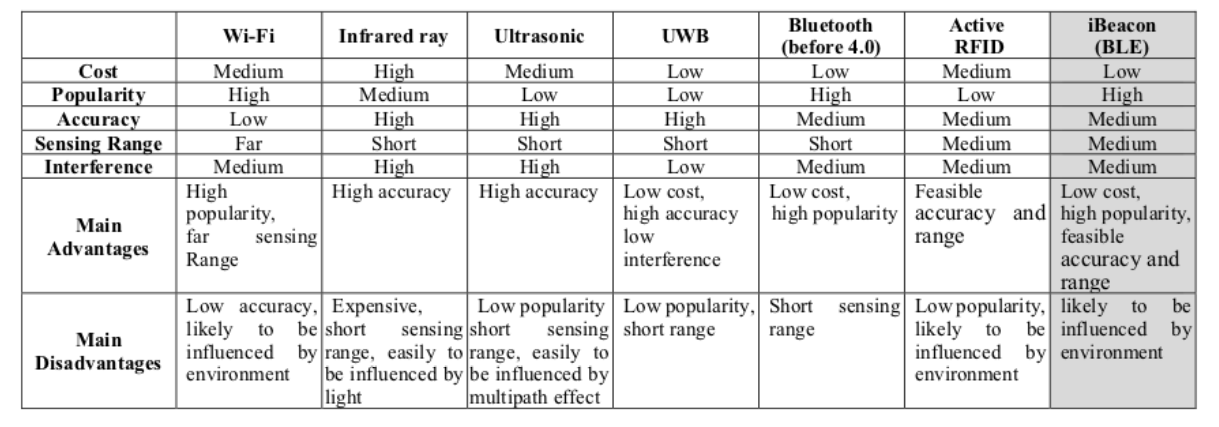
\includegraphics[width=1.0\linewidth]{media/comparison.png}
%	\caption{Comparison table}
%	\label{fig:translate_uml}
%\end{figure} 
%\end{center}

\begin{table}%[H]
    \centering
   
    \label{my-label2}
       \begin{tabular}{|p{30mm}|p{30mm}|p{30mm}|p{30mm}|}
 \hline
  & \textbf{Wi-Fi }&.        \textbf{NFC/RFID} &  \textbf{iBeacon} \\ [0.5ex] 
 \hline\hline
 \textbf{Cost} & Medium & Medium & Low \\ 
 \hline
 \textbf{Accuracy} & Low & Low & High \\
 \hline
 \textbf{Range} & Far & Medium & Far \\
 \hline
 \textbf{Advantages} & Highly popular, far sensing range & Feasible accuracy and range & Low cost, high accuracy and range. \\
 \hline
 \textbf{Disadvantages} & Low accuracy, influenced by environment & Low popularity, difficult to maintain & Likely to be influenced by environment. \\ [1ex] 
 \hline
    \end{tabular}
     \caption{Comparison of popular indoor positioning methods} {The important aspects we consider for this study to decide the method is the low cost and high accuracy feature \cite{sensing}. The range of the positioning method also played a huge role in order for us to consider the positioning method.}
\end{table}

\section{Understanding iBeacon Technology}
\label{iBeacon-tech}
\paragraph{}iBeacon is Apple’s implementation of Bluetooth low-energy (BLE) wireless technology to create a way of providing micro-location-based information and services to nearby smartphones supporting BLE. This allows mobile applications on a smartphone to determine when it has entered or left the region, along with an estimation of proximity to the smartphone. \\

Bluetooth 4.0 is proposed according to the Bluetooth technology standard set by the Bluetooth Special Interest Group (SIG) to achieve two-way transmission. When compared with traditional Bluetooth, Bluetooth 4.0 has the advantages of lower cost and lower energy. A button cell, such as CR2032 battery can make the device supporting Bluetooth Low Energy be operated for 1 to 2 years \cite{taiwan}. \\

iBeacon devices simply broadcasts its configured advertising packets in specific time intervals \cite{one}. Apple has standardized the format for BLE Advertising. In this format, a packet of information from a beacon consists of four main pieces of information. \\


\begin{figure}[H]
	\centering
	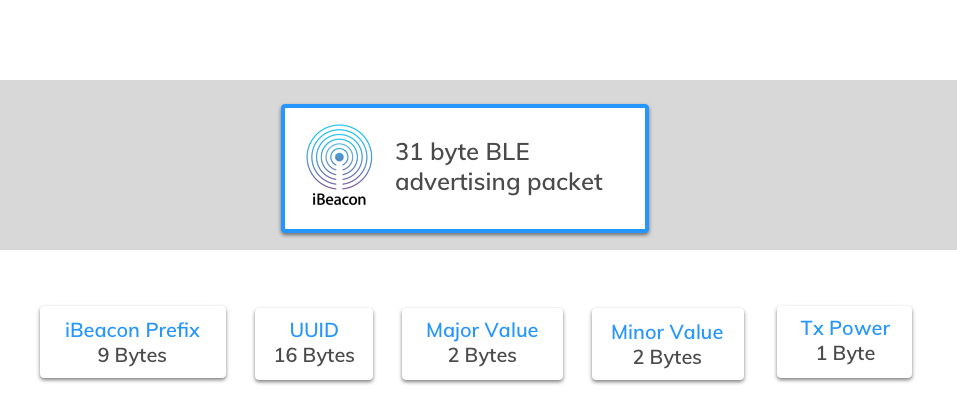
\includegraphics[width=1.0\linewidth]{media/ibeacon-format.jpg}
	\caption{iBeacon packet format}{The figure shows how the breakdown of the beacon information. The smartphone needs to read the UUID, Major and Minor to fetch related data to the beacon. Tx power is associated with the strength or range of the beacon}
	\label{fig:translate_uml}
\end{figure} 

\paragraph{}Breaking down the iBeacon information, there are five major parts: fixed iBeacon prefix; the proximity UUID: an identifier used to distinguish the beacons from other systems using similar bluetooth beacons; the major number can group a related set of beacons in an organization, such an exhibition hall in a museum or a floor in a store; the minor number can be used to identify individual beacons in specific areas because each beacon has a different minor number, by which we know where the user is exactly located. TX power, is used to determine how close the user is to a beacon \cite{beacons}. It can be presented either as an estimate (immediate/near/far/out of range) or it can be used to calculate more precise measurement in meters.
%
%\paragraph{}An iBeacon can be placed in around an item (goods, art works, or some places of a shop or institution) or a special areas, take the lobby or the hallway between two exhibition halls or between the exhibition hall and other area.


\paragraph{} 
\textbf{UUID}: This is a 16 byte string used to differentiate a large group of related beacons. For example, if National Park Services (NPS) maintained a network of beacons among all national parks, all national park beacons would share the same UUID. This allows NPS dedicated smartphone app to know which beacon advertisements come from NPS owned beacons. Example: E6FA79C7-804F-4742-863B-BD4D282ED9BA. \\

\textbf{Major}: This is a 2 byte string used to distinguish a smaller subset of beacons within the larger group. For example, if NPS had fifty beacons in a particular national park, all fifty would have the same Major. This allows NPS to know exactly which park its visitor is in. Example: A beacon with UUID E6FA79C7-804F-4742-863B-BD4D282ED9BA and a major number of 1101. \\

\textbf{Minor}: This is a 2 byte string meant to identify individual beacons. Keeping with the NPS example, a beacon at the front of the park would have its own unique Minor. This allows NPS’s dedicated app to know exactly where the visitor is in the park. Example: A beacon with UUID E6FA79C7-804F-4742-863B-BD4D282ED9BA, major number of 1101 and a minor number of 9901.\\

\textbf{Tx Power}: This is used to determine proximity (distance) from the beacon. TX power is defined as the strength of the signal exactly 1 meter from the device. This needs to be calibrated in advance to deployment. Devices can then use this as a baseline to calculate an estimate of distance between the beacon and the smartphone.  \\

\subsection{Existing applications implemented using iBeacon technology}

\begin{itemize}
	\item In a store, the retailer can understand shoppers’ interests by calculating the time spent by a shopper in front of a specific item in the store, and then, the application in shopper’s smartphone will show the other recommendation of related products \cite{beacons}.

\item The retailers can track shoppers behavior, for example, the shopper has seen the same goods in the other store of the same chain online and use with iBeacon technology to recommend those when visiting the store \cite{beacons}. The retailers can push the coupons information as well.

\item iBeacon technology brings many options for the retailers to send notifications of the items/events information to user's smartphone \cite{beacons}; to trace users interests or potential demands; to contextualize shoppers’ purchase tendency based on the user's history.

\item{} A study was conducted implementing iBeacons in the campus for the purpose of indoor positioning of the students and send out relevant information \cite{campus}.

\end{itemize}

\subsection{Operating range of iBeacons}
\paragraph{}iBeacon devices transmit its information to all devices that use this technology from a range of a few inches to more than 70 meters. The actual distance at which the device operates varies, depending on the environment. Just like all the radio waves, Bluetooth loses its power when it encounters obstacles \cite{demo}. All devices capable of supporting the Bluetooth 4.0 can take advantage of this system without the need of having to pair devices previously.

\subsection{Calculating distance between iBeacons, based on RSSI}
\paragraph{}The rate of signal strength will not be stable because of RF signal in actual obstacles in environment. So, there is no longer accurate correspondence between the RSSI and distance. Also, we need to purify the received data in order to reduce the correspoding positioning errors.

\paragraph{}We place iBeacon at a fixed position in the test environment. The mobile terminal detects the response of iBeacon signal strength, and we build out RSSI vector set based on the received signal, this set represents the RSSI vector is R=(R\textsubscript{1}, R\textsubscript{2}.....R\textsubscript{i}.....R\textsubscript{P}),where i is the signal strength of i-node RSSI, P is the total number of iBeacon. \cite{distanceTrack}

\paragraph{}We then repeatedly measure RSSI and averaging the values, the average value as the iBeacon RSSI value r=(r\textsubscript{1}, r\textsubscript{2} ,,,, r\textsubscript{i} ,,, r\textsubscript{m}), the formula is as follows:

\begin{equation}
RSSI = 1/m \sum_{i=1}^m RSSI \textsubscript{i}
\end{equation}

where m is the total number of collected RSSI vector at the coordinate points. This approach would correct the rather unstable distance of the beacon from the user. 


\section{RESTful web services}
\paragraph{} The mobile application developed communicates with the web-services such as Google Cloud Vision and Google Translation using Representational State Transfer (REST).  REST is an 
architecture that defines a set of rules to be used for creating web services \cite{rest}. Web services that conform to the REST architectural style, or RESTful web services, provide interoperability between computer systems on the Internet.

\paragraph{}By using a stateless protocol and standard operations, REST systems aim for fast performance, reliability, and the ability to scale, by re-using components that can be managed and updated without affecting the flow of other functions in the system as a whole, even while it is running in the background. In our system, we interact with Google Vision and Translation web-services through REST method. The response from these web-services is processed in the mobile application and appropriate messages are shown. A sample request and response for each web-services is shown in Sections \ref{vision} and \ref{translate}.

\section{Google Vision}
\label{vision}
\paragraph{}Google Cloud Vision is an image recognition technology that allows us to remotely compute the content of an image and to retrieve the information present in the media. By using Representational State Transfer (REST), called Google Cloud Vision API, we can use such technology within our own applications \cite{vision}. By using Google’s Cloud Platform to compute the content of an image through advanced machine learning processes, this solution allows us to extract relevant information from visual data, including image labeling, face and landmark detection, optical character recognition (OCR). It is possible to interact with Google’s Cloud Vision platform by using specialized REST API, called Google Cloud Vision API \cite{vision}.

\paragraph{}We propose to use such cloud-based software resources in order to achieve a system for people with understand signages and their environment in general. In particular for users who are visiting foreign countries, our solution may help them to interact with the environment and the things around them. In this paper, we focus on the OCR functionality of the Google Cloud Vision. We also discuss the implementation and integration of the Google Vision into our software solution, a mobile application we developed. The smartphone requires an Internet connection to submit the captured images to Google’s cloud platform. The response from platform is processed and displayed on the user's smartphone.

\paragraph{}The algorithm shown in Figure \ref{fig:vision} has been implemented in Javascript. In particular, here the request for Google Cloud Vision includes the TEXT DETECTION feature. A sample request and response is shown below:

\begin{figure}[H]
	\centering
	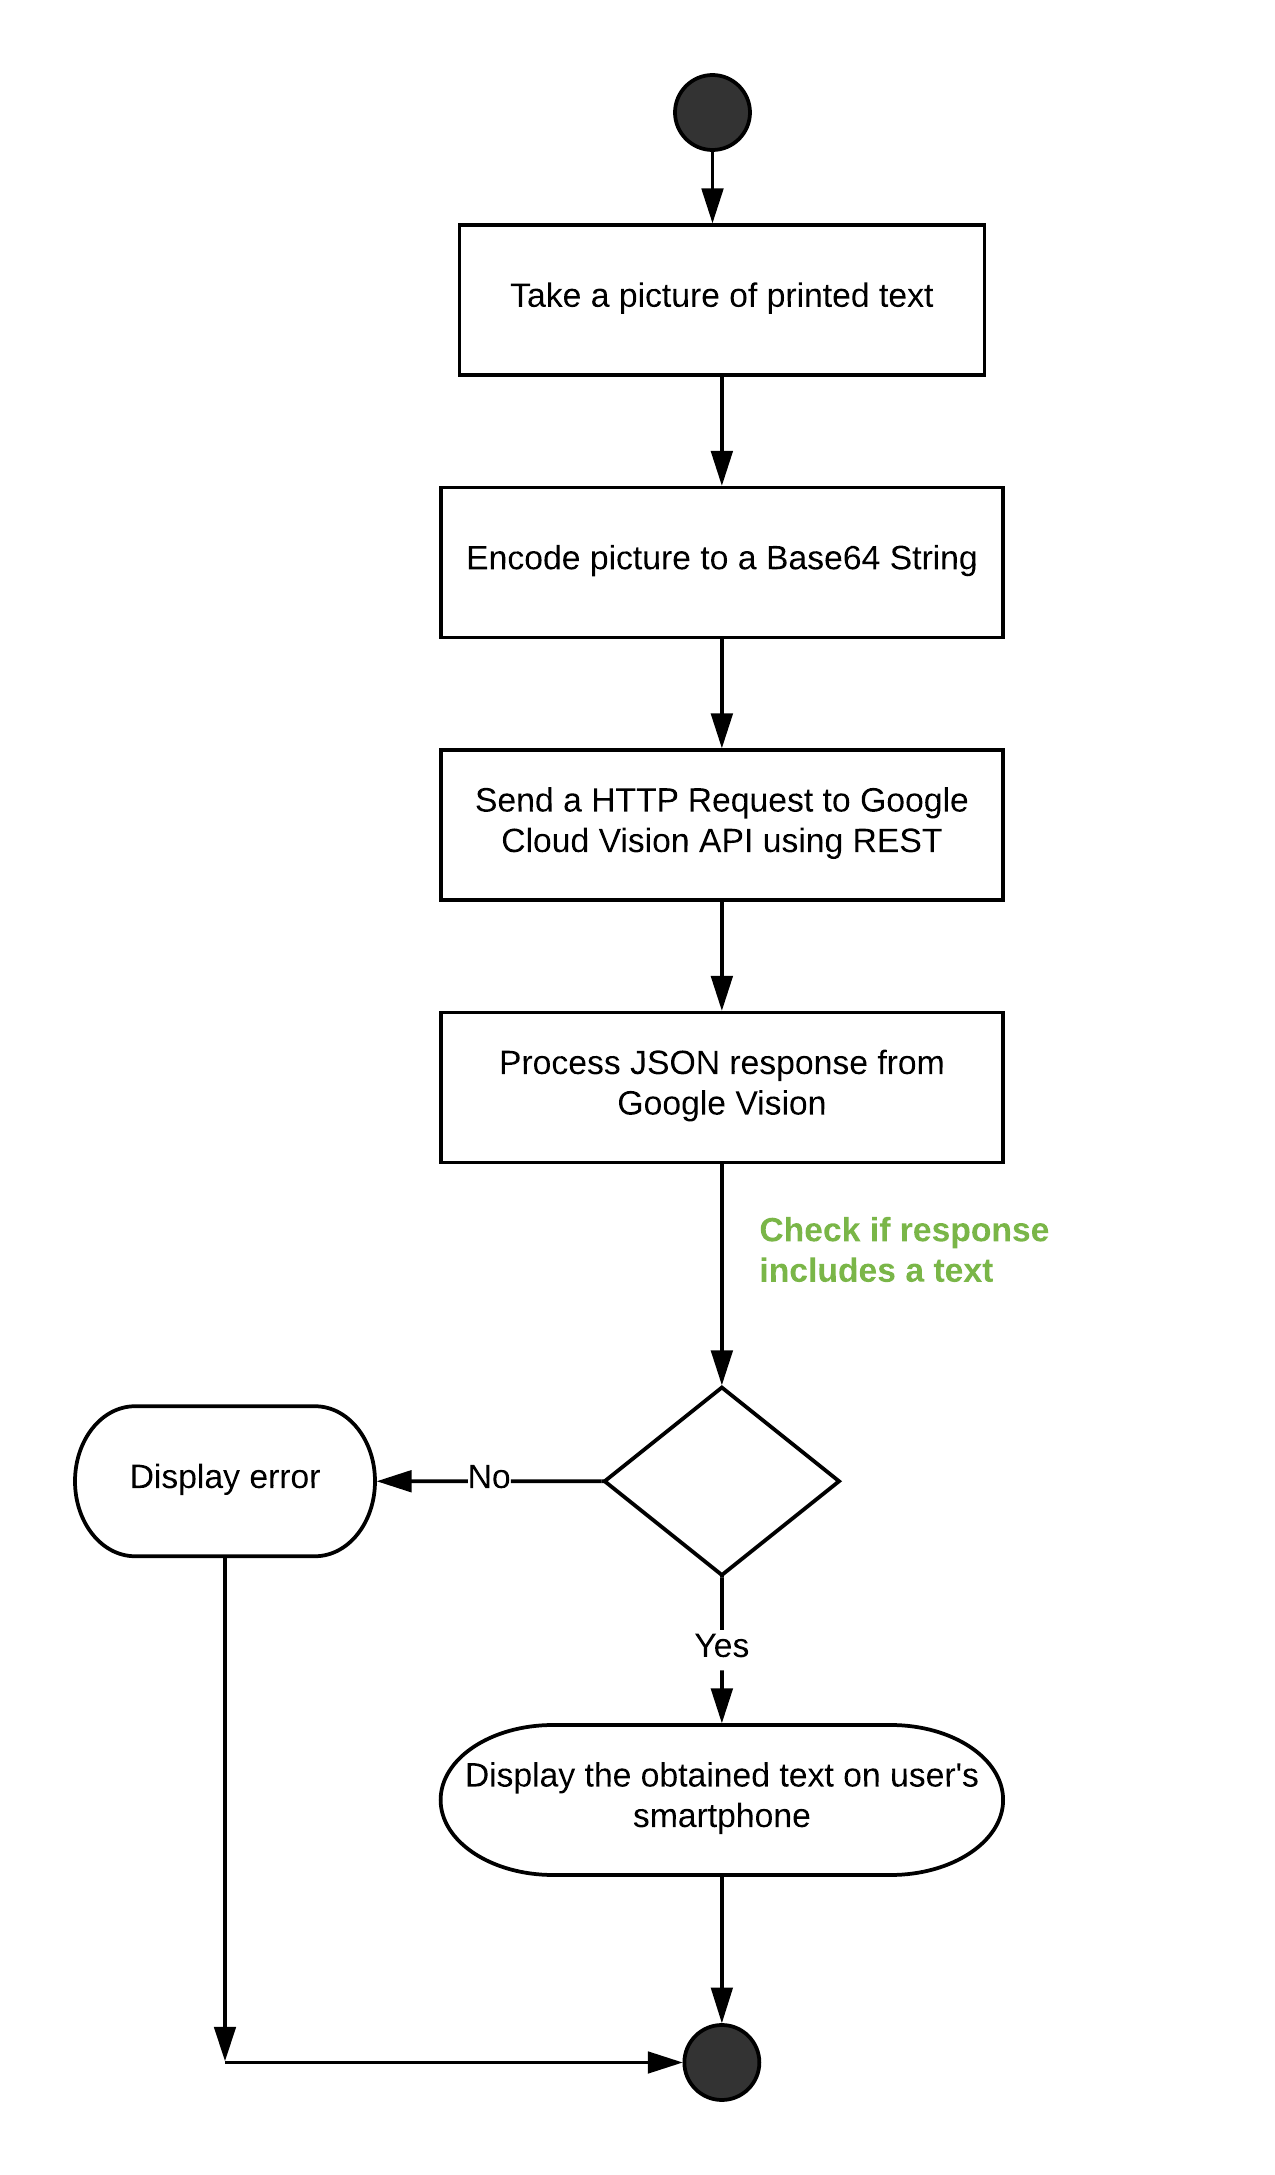
\includegraphics[width=0.75\linewidth]{media/VISION_API.png}
	\caption{Process flow diagram for Text Detection using Google Vision}
	\label{fig:vision}
\end{figure} 

\subsection{Sample Request}

\paragraph{}Let us consider the image shown in Figure \ref{fig:request_sample} as the source of the image. We use the Algorithm mentioned in Figure \ref{fig:vision} to extract the text from the image.

\begin{figure}[H]
	\centering
	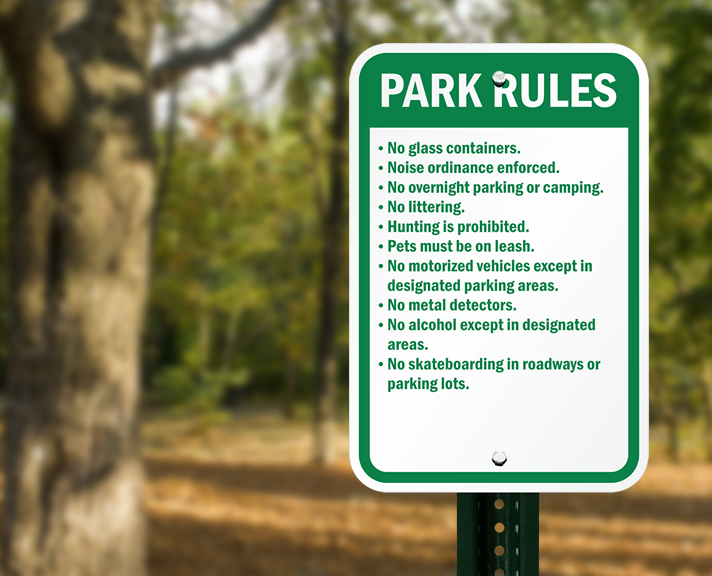
\includegraphics[width=1.0\linewidth]{media/request_sample.png}
	\caption{Example image for testing Google Vision API}
	\label{fig:request_sample}
\end{figure} 

We convert this image to a base64 encoded string using Javascript and specify in the headers of the REST API to use 'Text Detection' feature of Google's Cloud Vision API. A sample request is as shown below:

\begin{lstlisting}
{
	`requests':[{`image':{
	`content':`base64_encoded_string_of_image'
},	
	`features':[{`type':`TEXT_DETECTION',
	`maxResults':1}]}]
}
\end{lstlisting}

\subsection{Sample Response}

\paragraph{} In this section, we discussed the capabilities of Google Cloud Vision API and how we implement it into our system. We notice that the Vision Cloud API has analyzed the image, extracted the text and the same is returned to the device through the RESTful APIs.  

\paragraph{}The following is a sample response of extracted text from the Figure \ref{fig:request_sample}. It is a JSON object containing the image information.


\begin{lstlisting}
{
   
   `responses': [{
	`textAnnotations': [{
	`locale': `en',
	`description': `Pedestrian access only beyond this point',
	`boundingPoly': {
	`vertices': [
		{`x': 327,`y': 412},{`x"': 1158,`y': 412},
		{`x': 1158,`y': 680},
		{`x': 327,`y': 680}
		]}
	  }]
  }]
}
\end{lstlisting}


\section{Google Cloud Translation}
\label{translate}

\paragraph{}Google Translation API provides a simple application program interface (API) for translating any string/text into any supported language using the inbuilt Neural Machine Translation. It is highly responsive, so applications can integrate with Translation API for fast, easy translation of source text from the source language to a target language (such as Spanish to English). Language detection feature is also supported in cases where the source language is not known. The underlying technology is updated constantly to include improvements from Google research teams, which results in better translations and new language pairs.

\paragraph{}Translation API supports more than one hundred different languages, which makes it an ideal choice for us to use in this study. Translation API can be accessed using REST APIs. We extract text from the printed signages using Google Cloud Vision API, we then send the text to Google Translate API and convert it into the user's desired language.

\paragraph{}Figure \ref{fig:translate_uml} describes the process of language translation in our system. We obtain the text from the printed media using Google Vision API as mentioned in Section \ref{vision}. We then pass the obtained text to Google Cloud Translation API with the preferred language in the headers of REST API. The response from the Google Translate is then displayed in the user's smartphone. A sample request and response is shown below:

\begin{figure}[H]
	\centering
	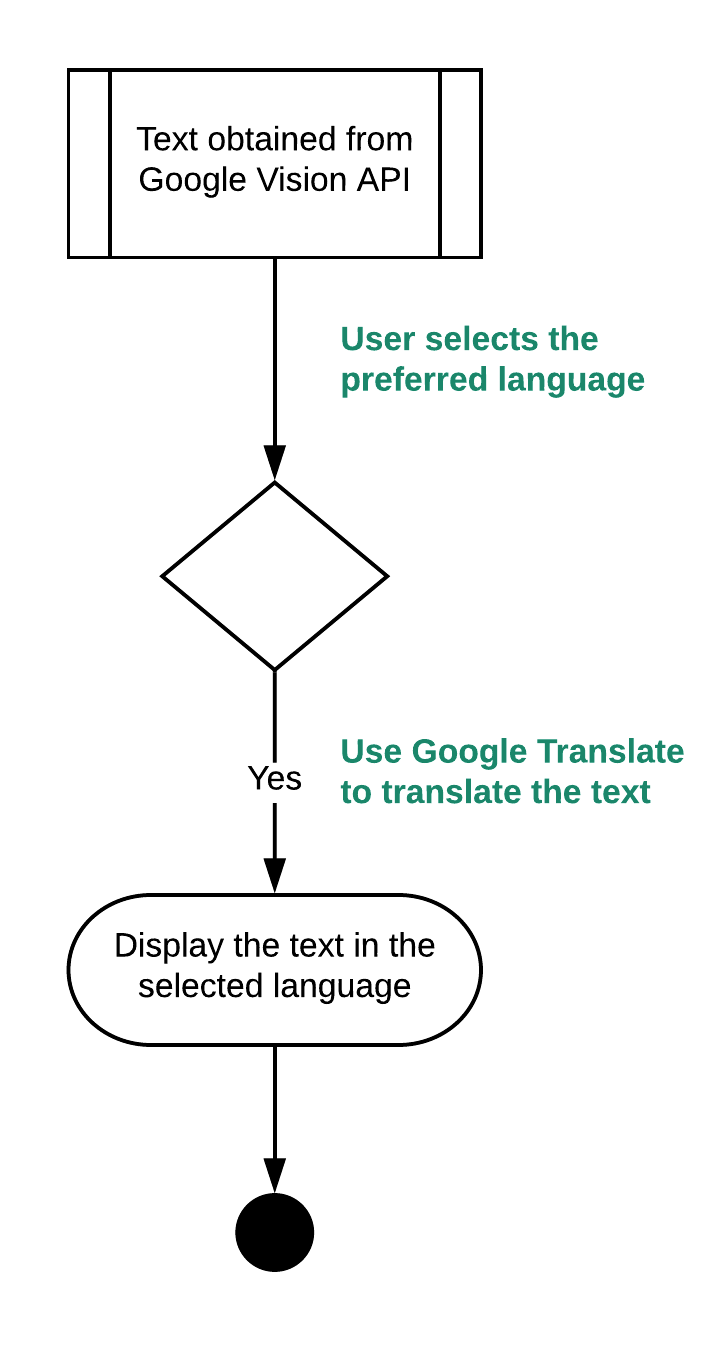
\includegraphics[width=0.5\linewidth]{media/Translate.png}
	\caption{Process flow diagram using Google Translation}
	\label{fig:translate_uml}
\end{figure} 

\subsection{Sample Request}

\paragraph{}The below code segment shows how to use Google Cloud Translate API using REST APIs using Javascript. Developers should replace their own Google API Key at  API-KEY-HERE. The target language to be translated is passed under 'target' parameter of the REST API. 

\paragraph{}We use javascript to interact with Google Translation API as follows:

\begin{lstlisting}
    fetch(`https://translation.googleapis.com/language/
    translate/v2?key=`API_KEY', {
      method: `POST',
      headers: {
        `Accept': `application/json',
        `Content-Type': `application/json',
      },
      body: JSON.stringify({
        q: `text_to_be_translated',
        target: `target_language'
      })
    })
    .then(data => data.json())
    .then(res => this.cleanText(res))
    .catch(err => (err))
  }
\end{lstlisting}

\subsection{Sample Response}

\paragraph{} Google Cloud Translation processes the requests, determines the text to be translated  and the target language. It then responds with a JSON object containing the translated text. All these is communicated to the application through RESTful APIs. A sample response is shown below:

\begin{lstlisting}

{
  `data': {
    `translations': [
      {
        `translatedText': `translated_text_here'
      }
    ]
  }
}
\end{lstlisting}

% Algorithm


\section{Algorithm}

\paragraph{}The below pseudo-codes show the algorithms involved in our system. The system constructed for the study runs both the below algorithms in the background. For convenience, we have divided the algorithm into 2 sections, one for digital signage and one for printed signages. 


\paragraph{}Algorithm 1 shows the pseudo-code for scanning iBeacons. The system built in the study scans for beacons in the background. When the beacons are found, the mobile application reads the parameters of each beacon and queries the database in the server with the parameters. If data is found in the server, the mobile application processes the data and displays appropriate signage information. The user can then choose to translate the data into his preferred language using Google Translation.

\begin{algorithm}
\caption{Pseudocode for digital signages}\label{euclid}
\begin{algorithmic}[1]
\Procedure{Scan for iBeacons}{}\label{omne}
\If {iBeacons found}
	\BState \emph{loop}: 
\State 	acquire RSSI info of beacon 
\State 	calculate and display distance of beacon
\State	query beacon parameters with server database

\If {data exists}
	\State fetch and display data
	
	%\State \textbf{goto} \emph{loop}.
	
	\Procedure{User selects preferred language}{}
	\State fetch selected language
	\State send the text and selected language to Google translation
	\State fetch and display text in user's preferred language
\EndProcedure

\EndIf
% \State $counter \gets counter+1$.
%\State \textbf{goto} \emph{loop}.
\EndIf
\EndProcedure
\end{algorithmic}
\end{algorithm}


\paragraph{} Algorithm 2 shows the pseudo-code for extracting text from printed signages and then translating them to preferred language. The system listens to the event of image capture from smartphone camera or image upload from the camera roll. On this event, the system converts the image into a base64 encoded string and communicates with Google Cloud Vision using REST method. If the server is successful in extracting text from the image, it responds with a JSON file containing the extracted text. The mobile application then processes the data and displays the extracted text. The user can then choose to translate the data into his preferred language. On selecting a language, the system then sends both the extracted text and selected language to Google Translation using REST method. On successful translation, the system then displays the information in user's selected language on the mobile application.

\begin{algorithm}
\caption{Pseudocode for printed signages}\label{euclid}
\begin{algorithmic}[1]
\Procedure{User captures an image of signage}{}
\State convert image to Base64 encoded string
\State send the image to Google cloud vision 
\If {text returned}
\State 	parse the response and display text
\Procedure{User selects preferred language}{}
	\State fetch selected language
	\State send the text and selected language to Google translation
	\State fetch and display text in user's preferred language
\EndProcedure
%\State \textbf{goto} \textbf{procedure}.
\EndIf
\EndProcedure
\end{algorithmic}
\end{algorithm}


%System 

\section{System Design}
\label{system}
\paragraph{}In this study, a prototype of multilingual information service system was designed and constructed. 3 beacons were configured and placed next to each of the 3 signage in the university campus. These beacons continuously broadcast their UUID, Major and Minor. A mobile application was constructed to listen to these beacons. The mobile application leverages the smartphone’s bluetooth technology to listen to the beacons.

\paragraph{}The relevant information of the signage for each beacon is stored in a database using Google Firebase, a cloud storage. Once the mobile application detects a beacon, it makes a call to the cloud, passing the detected beacon configuration to get the appropriate information of the signage using REST APIs. The information returned from the cloud is then translated to required languages using the Google Translate API and displayed on the user’s smartphone.

\paragraph{}Figure \ref{fig:system} below gives an overview of different processes in our system.

\begin{figure}[H]
	\centering
	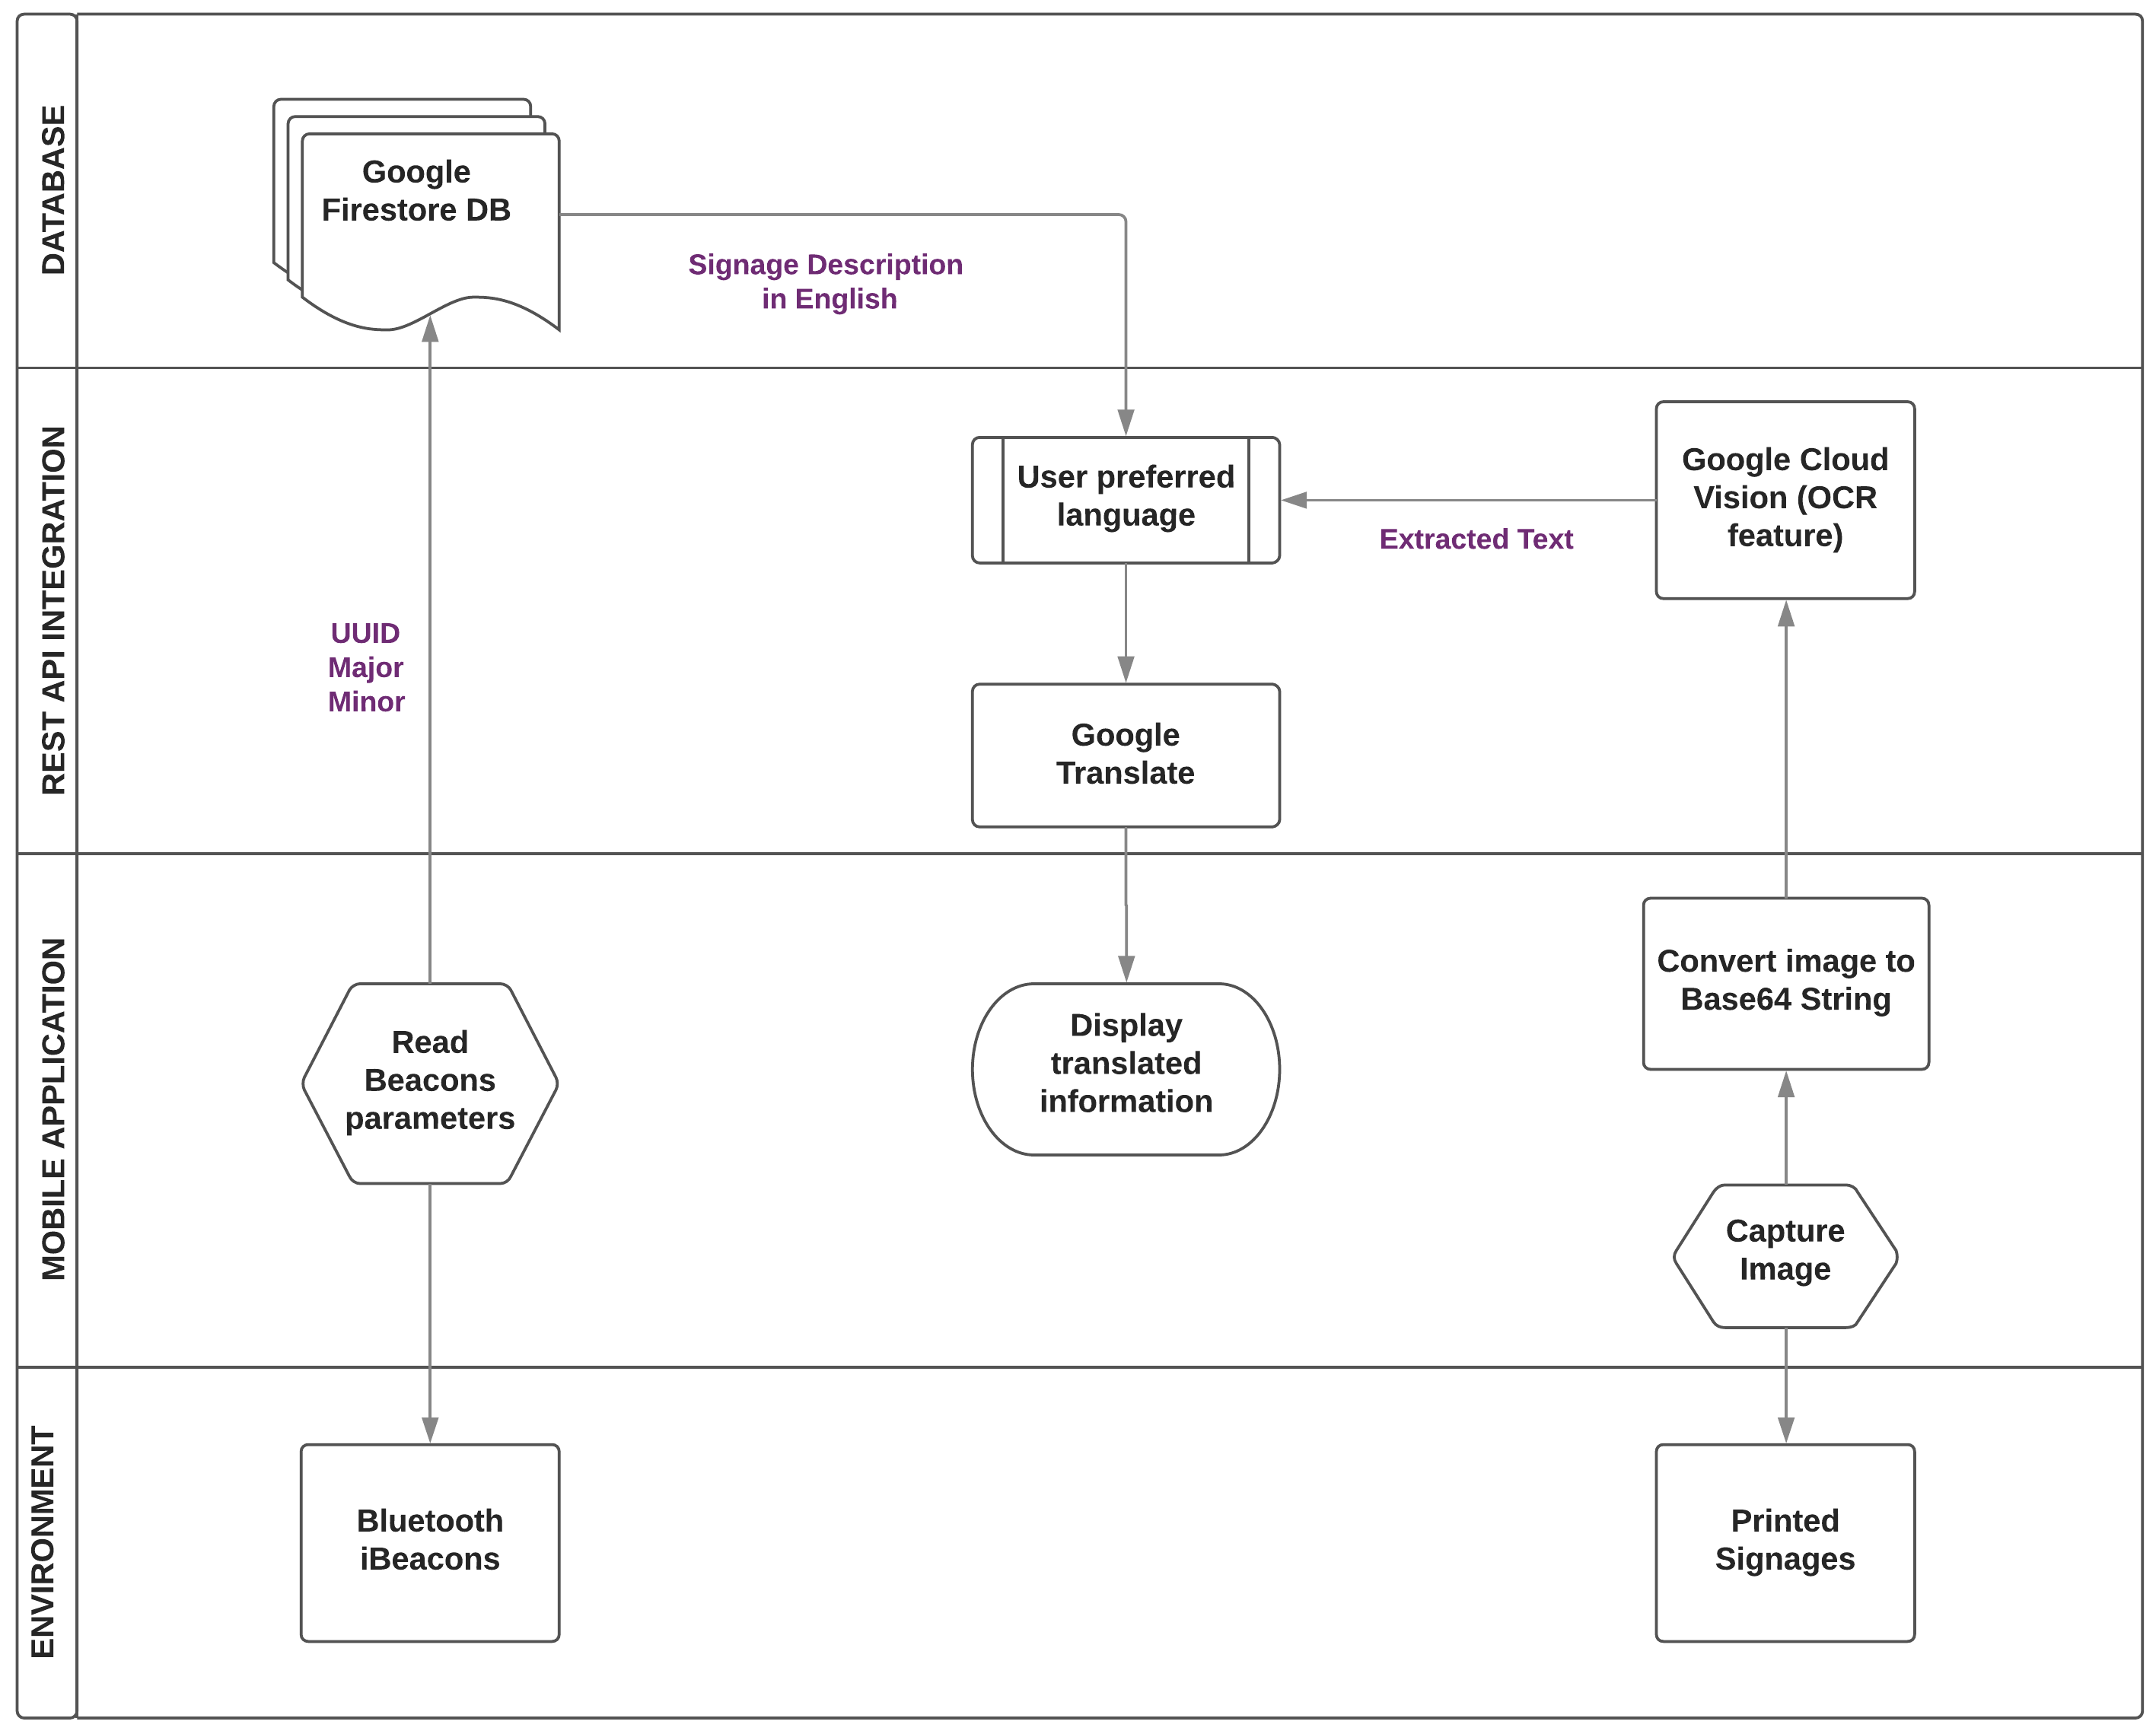
\includegraphics[width=1\linewidth]{media/Architecture-3.png}
	\caption{System design process flow diagram. The diagram shows all the individual components of the system and how it is integrated together to achieve the objective.}
	\label{fig:system}
\end{figure} 

\subsection{Environment setup}
\label{env}
\paragraph{}To evaluate the system, we constructed a combination of digital signages and printed signages were placed around the California State University, Channel Islands (CSUCI) campus. Each signages were placed at least 100 meters apart. For optimal working of the system, the beacons need to be placed 15 meters apart.

\subsubsection{Digital Signages}
\paragraph{}The digital signage was set up using the bluetooth iBeacons. Each iBeacon is mounted on individual signages in the campus. The beacons are powered by individual CR2032 lithium-ion coin batteries. The users used the iPhone 6s in which the application program that reacts with the iBeacon signals. The parameters of the beacons, which are discussed in the Section \ref{iBeacon-tech} can be configured only by the administrator of the mobile application. To evaluate the system, we use 3 beacons. Below are the configurations of each beacon used in the study.

\begin{lstlisting}
UUID: E6FA79C7-804F-4742-863B-BD4D282ED9BA
Major: 1111
Minor: 9991
\end{lstlisting}

\noindent\rule{13cm}{0.4pt}

\begin{lstlisting}
UUID: E6FA79C7-804F-4742-863B-BD4D282ED9BA
Major: 1111
Minor: 9992
\end{lstlisting}

\noindent\rule{13cm}{0.4pt}

\begin{lstlisting}
UUID: E6FA79C7-804F-4742-863B-BD4D282ED9BA
Major: 1111
Minor: 9993
\end{lstlisting}

\subsubsection{Printed Signages}
\label{printed-signages}
\paragraph{}To evaluate our solution of translating the signages without the iBeacons, we printed out commonly used  signages in Spanish language and placed them around the CSUCI campus. 

\subsection{Mobile application}

\paragraph{}
To discover the beacons from the smartphone, we have designed and developed a mobile application. This mobile application is built using React native and Javascript. The mobile application uses Google Cloud Vision to detect the printed text using the smartphone camera. The Google Cloud Vision API detects the printed information using OCR feature as mentioned in Section  \ref{vision}. This text can be converted to any language using Google Cloud Translation API, discussed in Section \ref{translate}. The mobile application interacts with these APIs using RESTful method. To improve the efficiency and user-experience, we used both iBeacon monitoring and ranging to discover and interact with the beacons.


\subsubsection{Background Monitoring}
\paragraph{}Beacon monitoring is similar to geofencing, i.e., a virtual barrier that is usually defined using a set of geographic coordinates. In case of iBeacon, an area is defined by the range of one or more beacons. Moving and out of the area under the umbrella triggers ’enter’ and ’exit’ events, which the mobile application can listen and trigger events accordingly. The smartphone will keep scanning for the beacons at all times even if the application is not running in the foreground, and even if the smartphone is 'locked'. Once an ’enter’ or ’exit’ happens, iOS will launch the application into the background (if needed) and execute some code for a few seconds to handle the event.

\subsubsection{Beacon Ranging}
\paragraph{} Ranging refers to the process of scanning for any nearby beacons on the foreground and delivers results as and when the environment changes. With monitoring, our application will be notified whenever the user enters and exits the terminal. Ranging for the exact same region, will provide us with the full list of matching beacons currently in range - with the UUID, major, and minor values.

\subsubsection{Development stack}
\paragraph{} The mobile application was developed after evaluating all the major development tools and technology present in the current market. The main goal is to develop the system, keeping performance and scalability in mind. Also, we want to make sure the system works efficiently on both iOS and Android platforms. Below is the development stack we used to develop the mobile application:

\begin{itemize}
  \item \textbf{React Native:} To develop the front end of the mobile application. The advantage of using React Native is it helps us to develop for both Android and iOS with the same codebase. Also, React Native is efficient in terms of performance.
  
   \item \textbf{JavaScript:} We used JavaScript to interact with the web-services such as Google Vision and Google Translate. It makes it efficient to convert the captured images into Base64 encoded string and pass it in the headers of the request. Also, JavaScript makes it easier to process/parse the JSON response from the web-service and display it on the front-end using React Native. We use JavaScript also to communicate with the Google Firestore database to query and retrieve data.
  
      \item \textbf{Camera:} To access the smartphone camera, we included a library called 'react-native-camera'. This extends the functionality of camera in terms of fragments and hence makes it easier to listen to the camera events and implement our logic where necessary.
      
        \item \textbf{Bluetooth:} Our system needs access smartphone's bluetooth module to discover the iBeacons. To check the state of Bluetooth, we included 'react-native-bluetooth-state' library. This helps us determine the bluetooth status of the smartphone, whether 'on' or 'off' and display appropriate messages to the user.
        
        \item \textbf{Beacon Manager:} To discover iBeacons from the smartphone, we integrated 'react-native-beacons-manager' library into React Native. This library helps us scan for the beacons and listen to changes of the beacon signal strength. The library also supports 'background ranging' and 'foreground monitoring' of the beacons, meaning it helps us scan for the beacons even when the application is running in background. 
      
      \item \textbf{Xcode:} To build and run the application on the iOS device, we need an Integrated Development Environment (IDE). Xcode is an IDE that can be used to run the developed mobile application on the iOS device. The source code for the implementation could be found at \cite{git}.
      
 \end{itemize}
 
 
 \subsubsection{Screenshots}
 
\paragraph{}The below figures show the screenshots from the constructed mobile application. Figure \ref{fig:landing} shows the Landing screen of the application. The user sees this screen on opening the application. The Home page has the following functionalities: 

\begin{itemize}
	\item Capture image of a physical signage
	\item Scan for digital signages around. If found, display the image, title and the distance of the digital signage from the user.
	\item The user can also upload an image form camera roll of the smartphone and extract text from it. 
	\item The user can choose to type a text and convert it into any language
\end{itemize}


 \begin{figure} [H]
\centering
\begin{minipage}{.5\textwidth}
  \centering
  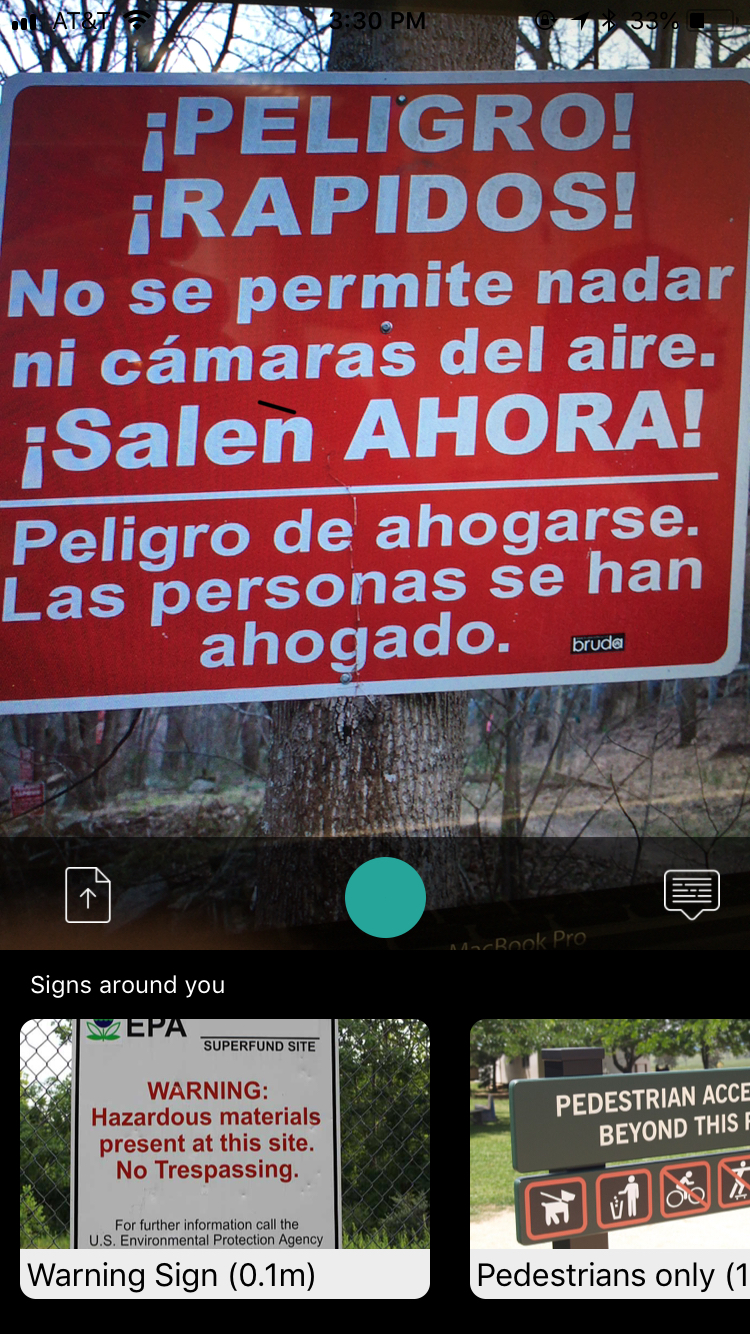
\includegraphics[width=0.9\linewidth]{media/1.jpg}
  \caption{Home page}
  \label{fig:landing}
\end{minipage}%
\begin{minipage}{.5\textwidth}
  \centering
  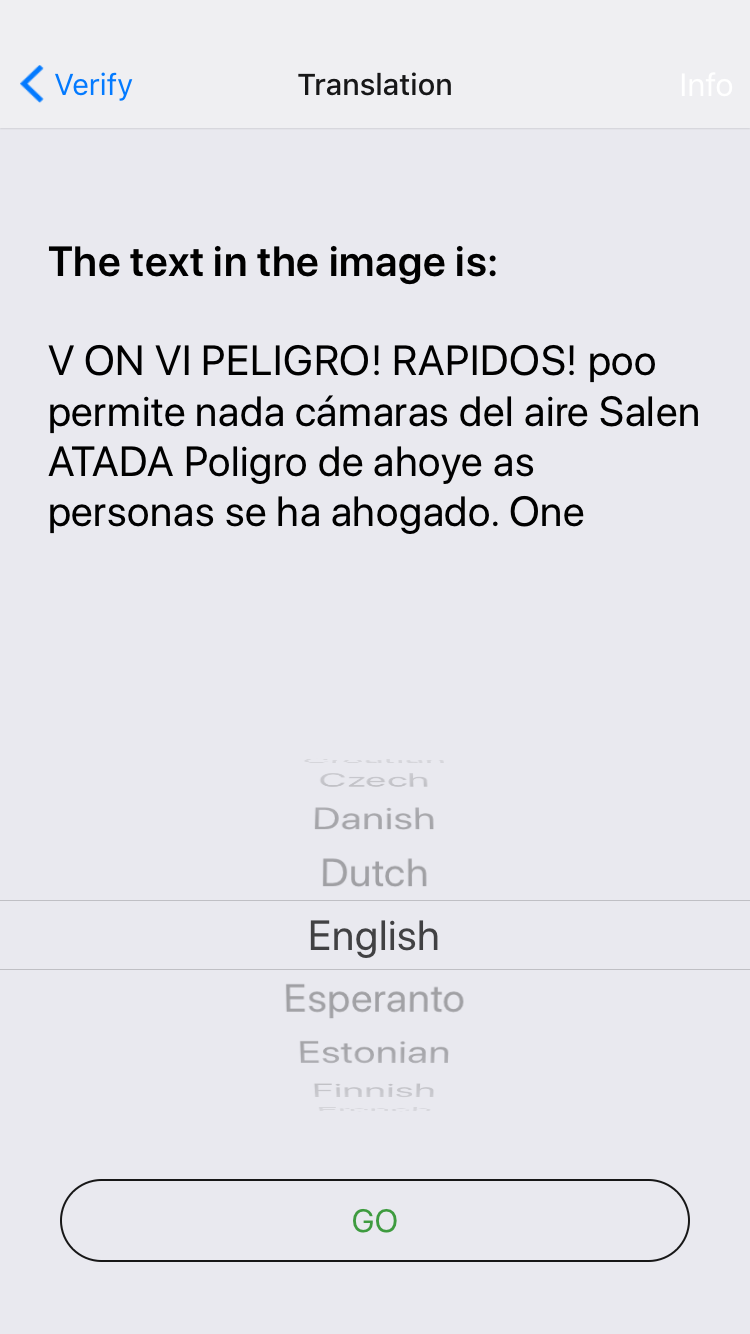
\includegraphics[width=0.9\linewidth]{media/2.PNG}
  \caption{Text extraction}
  \label{fig:ocr}
\end{minipage}
\end{figure}



\paragraph{}Figure \ref{fig:ocr} shows the text extracted from the image captured on Figure \ref{fig:landing}. This screen is presented to the user right after capturing an image of a physical signage. We convert the captured image into Base64 string and pass it to Google Cloud Vision using REST and extract the text from the image. The screen on Figure \ref{fig:ocr} has the below functionalities: 

\begin{itemize}
	\item Display the extracted text from the image
	\item The user can choose to translate the extracted text to any of the supported language. 
\end{itemize}



\paragraph{}Figure \ref{fig:translated} shows the text translated into Spanish. This is the same text extracted from Figure \ref{fig:landing}. The extracted text is shown on Figure \ref{fig:ocr}. This screen is presented to the user after the user chooses a language and taps on the 'GO' button. We listen to the event, capture the language selected and send a request to Google Translation API using web-services. The screen on figure \ref{fig:translated} has the below functionalities:

\begin{itemize}
	\item Display the translated text in user's preferred language.
	\item Share the translated text using Share button.
	\item Capture another image of a physical signage.
	\item Go back to landing page.
\end{itemize}

\paragraph{}An important design consideration was to allow the option to share the translated text in any form. Figure \ref{fig:share} shows the Share feature we integrated so the user can record the translated text and share them with friends and family who might need the information. In our system, the user can choose from the multiple options to share the translated text. The default options of the iOS applications include e-mail application, messaging application, notes application etc. 


 \begin{figure} [H]
\centering
\begin{minipage}{.5\textwidth}
  \centering
  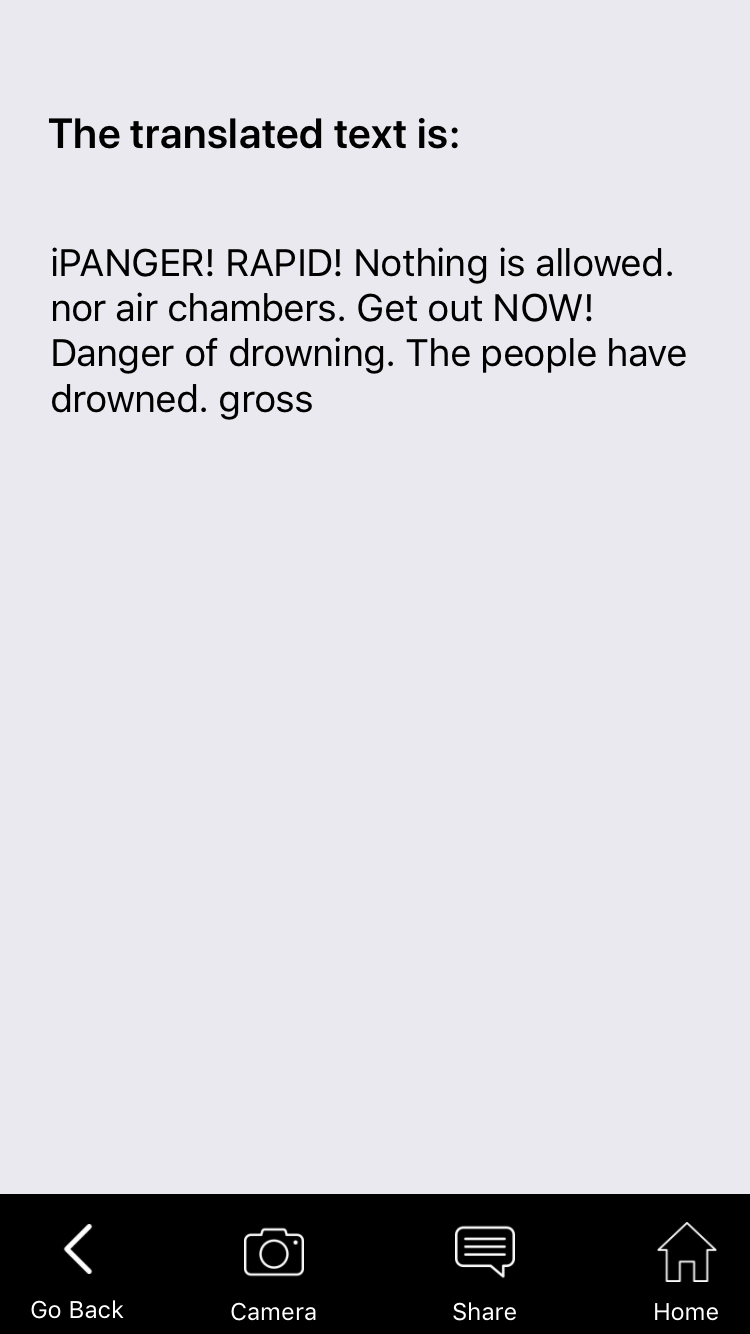
\includegraphics[width=0.9\linewidth]{media/3.PNG}
  \caption{Translated text}
  \label{fig:translated}
\end{minipage}%
\begin{minipage}{.5\textwidth}
  \centering
  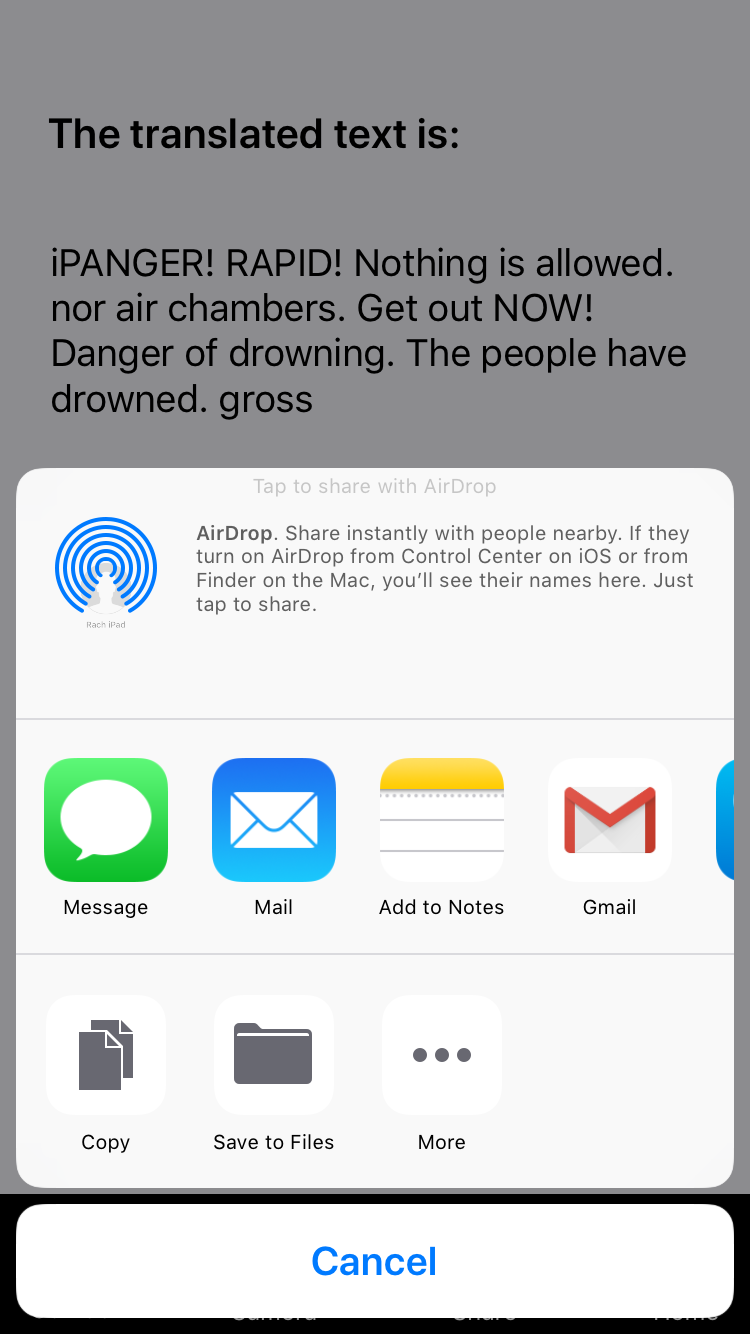
\includegraphics[width=0.9\linewidth]{media/4.PNG}
  \caption{Share text feature}
  \label{fig:share}
\end{minipage}
\end{figure}


\paragraph{} Since our primary users of our application are non-native visitors, we feel there is a strong need for them to communicate day-to-day for critical information in their native language. To achieve this in our system, we implemented a 'type and translate' feature. Figure \ref{fig:type} shows the screenshot of the 'type and translate' feature. The user can type in text in any language and choose to convert it into any of the supported languages. 
\begin{figure}[H]
	\centering
	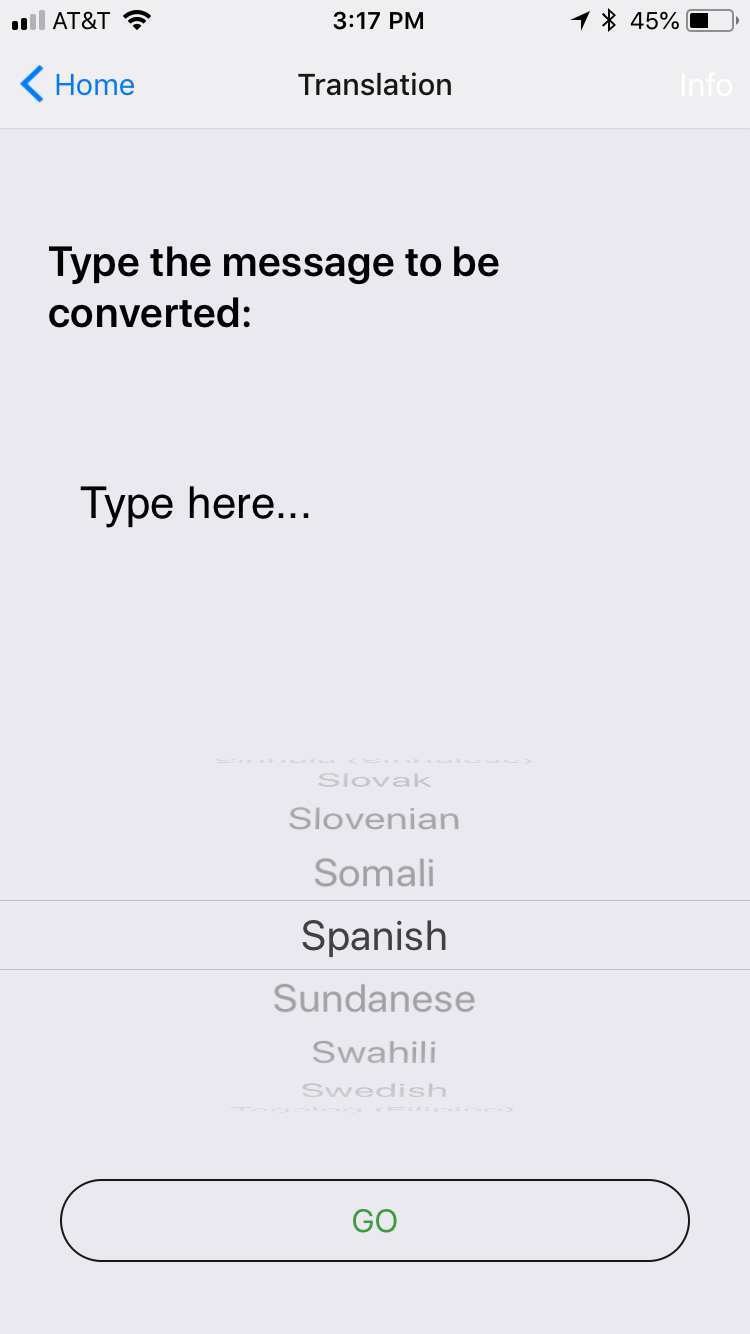
\includegraphics[width=0.5\linewidth]{media/5.PNG}
	\caption{Type and translate text feature}
	\label{fig:type}
\end{figure} 

\paragraph{} The user lands on the screen shown in Figure \ref{fig:beaconDetails} after tapping on any of the digital signage thumbnail. When the user taps on a particular signage, the system screen fetches the pre-configured information and media from the database and displays them on this screen. This screen displays the image of the signage, the title and the description of the signage in English. This component  has the below functionalities:

\begin{itemize}
	\item Fetch and display the appropriate data (media, title and description) from the database.
	\item Provide the user with the option of translating the information into supported languages.
\end{itemize}

\paragraph{}The screen in Figure \ref{fig:beaconTranslate} is shown when the user taps on 'Translate' button from screen in Figure \ref{fig:beaconDetails}. The information of the digital signage is passed to this screen. Now, the user can translate the text into any supported language. This component is capable of the below functionalities:

\begin{itemize}
	\item Display the beacon information.
	\item Provide the user with the option of translating the information into supported languages.
\end{itemize}


 \begin{figure} [H]
\centering
\begin{minipage}{.5\textwidth}
  \centering
  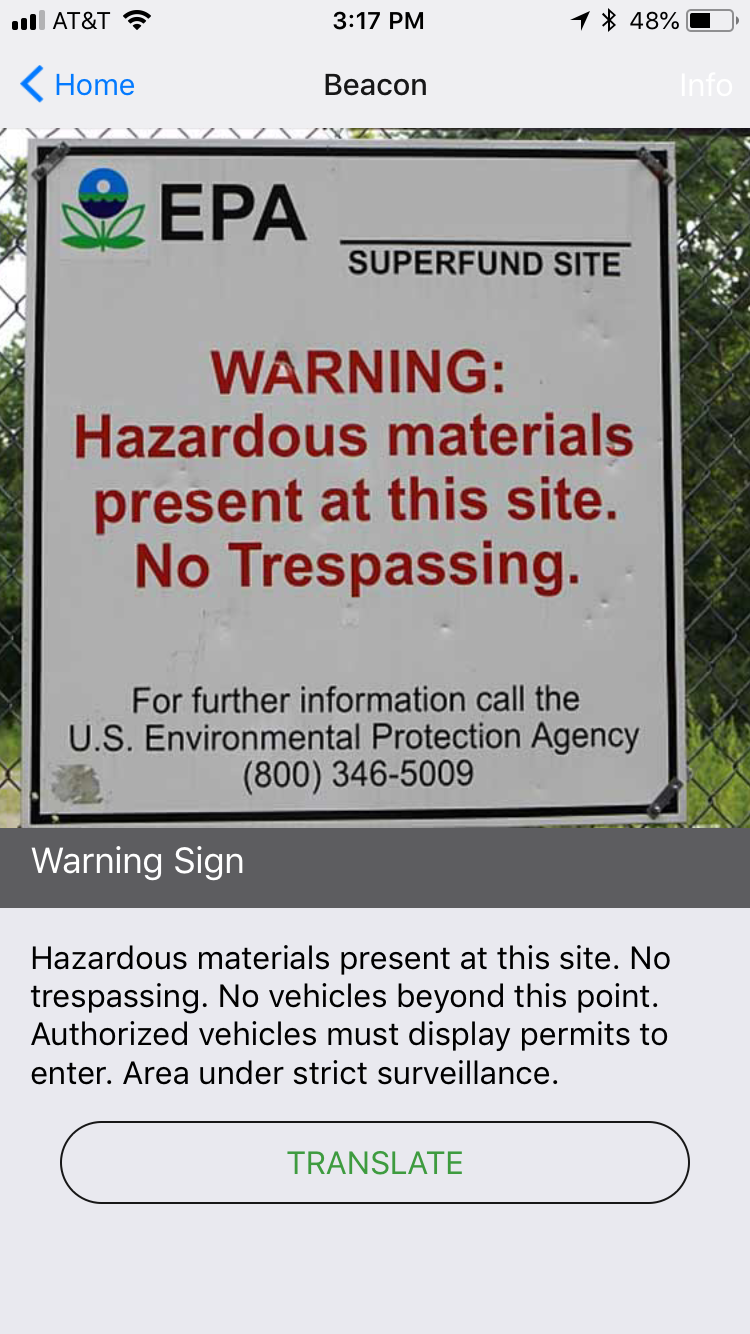
\includegraphics[width=0.9\linewidth]{media/beacon.PNG}
  \caption{Digital Signage}
  \label{fig:beaconDetails}
\end{minipage}%
\begin{minipage}{.5\textwidth}
  \centering
  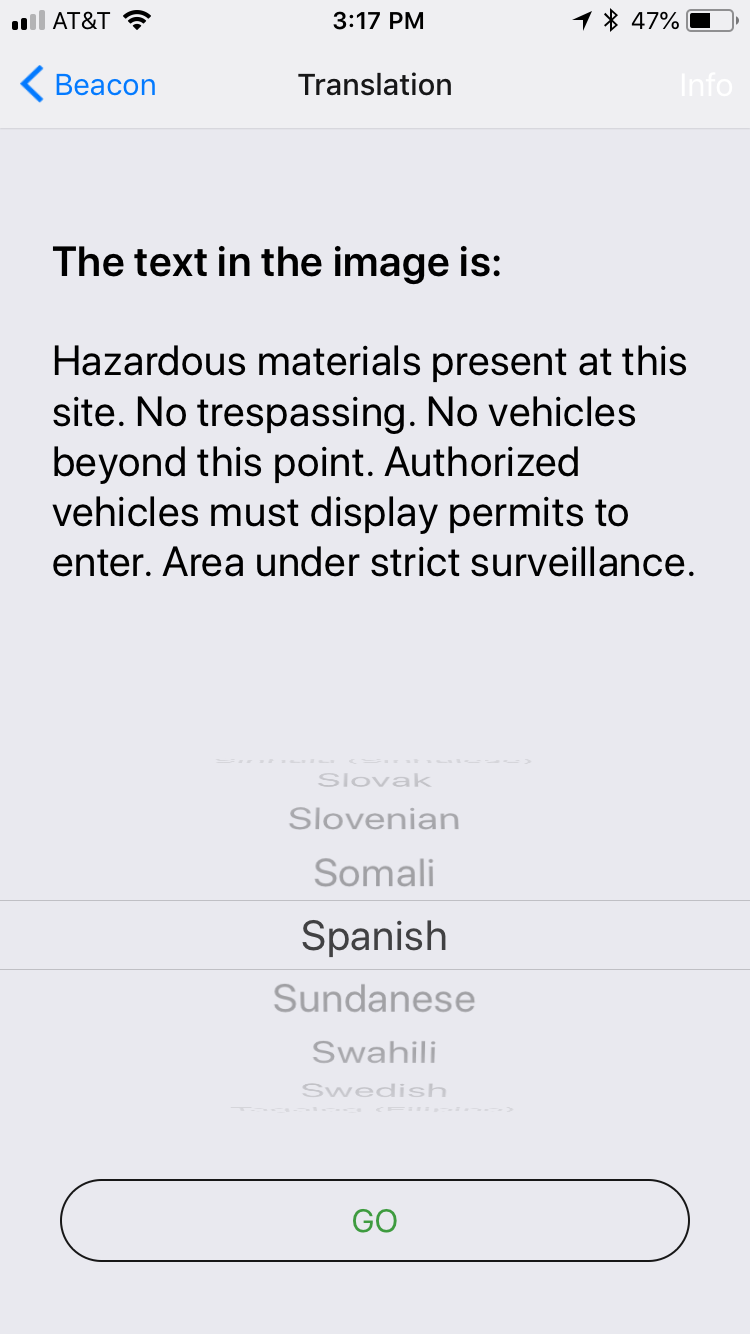
\includegraphics[width=0.9\linewidth]{media/beacon2.PNG}
  \caption{Translate feature}
  \label{fig:beaconTranslate}
\end{minipage}
\end{figure}


\paragraph{}Figure \ref{fig:beaconSpanish} is shown when the user selects a language and taps on 'Go' button from Figure \ref{fig:beaconTranslate}. The information of the digital signage is passed to this screen. Now, the user can translate the text into any supported language. This component is capable of the below functionalities:

\begin{itemize}
	\item Display the translated text in user's preferred language.
	\item Share the translated information.
	\item Go back to landing page.
\end{itemize}




\begin{figure}[H]
	\centering
	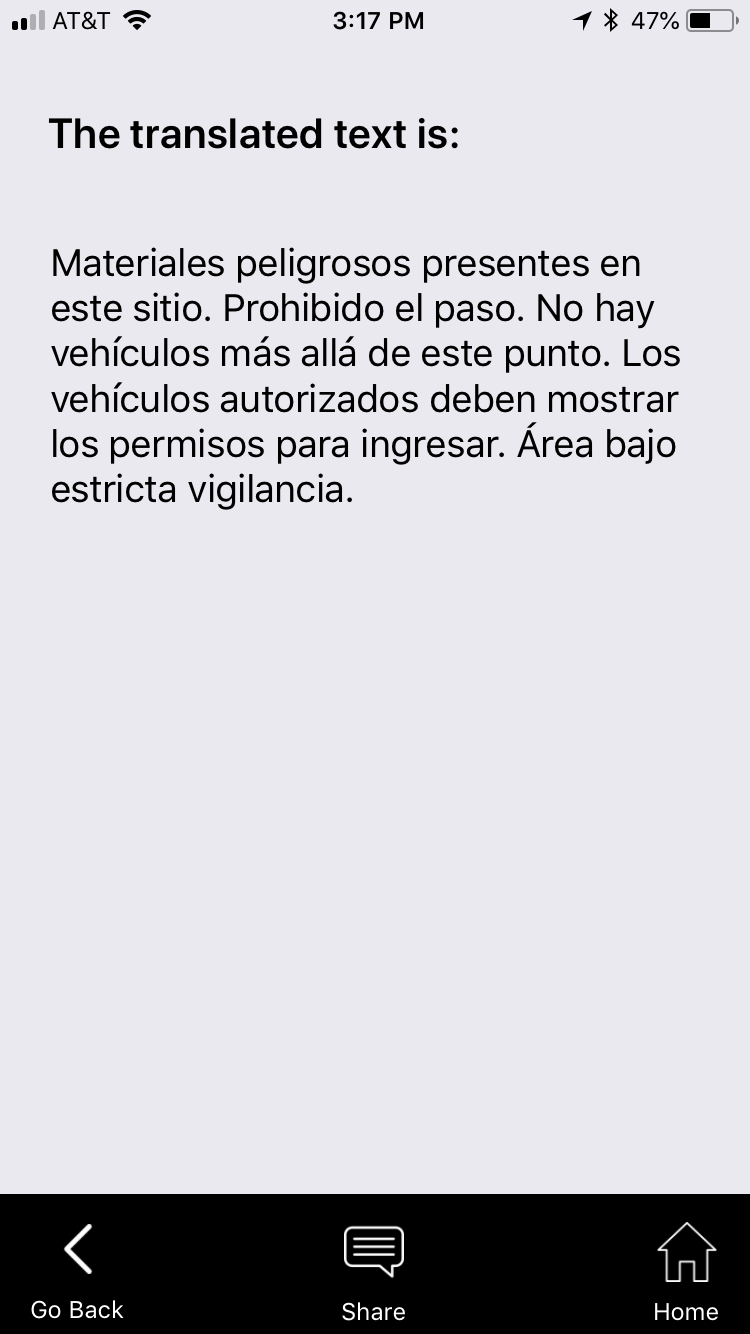
\includegraphics[width=0.5\linewidth]{media/beacon3.PNG}
	\caption{Text translated to Spanish language}
	\label{fig:beaconSpanish}
\end{figure} 






\subsection{Database}
\label{database}
\paragraph{}To store the information of each signage in a database, we chose Google Cloud Firestore. Cloud Firestore is a flexible, scalable database for mobile, web, and server development from Firebase and Google Cloud Platform \cite{firebase}. It keeps the data in sync across applications through realtime listeners and offers offline support for mobile and web so we can build applications that work regardless of network latency or Internet connectivity \cite{firebase}. Google Firestore is free of cost for less than 50 simultaneous connections to the database, which is a right fit for the study.

\begin{figure}[H]
	\centering
	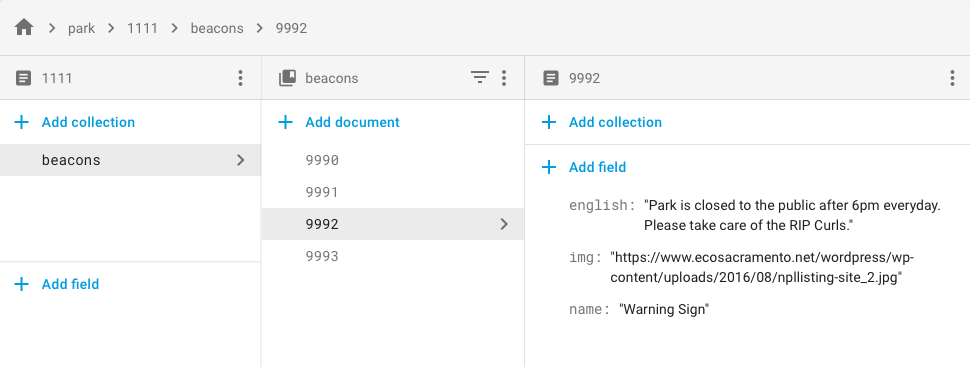
\includegraphics[width=1\linewidth]{media/db.png}
	\caption{Database Schema}{Database schema has been designed in a way that it is very easy to scale and use the system for any physical environment. The UUID is on top level of the schema and the Major and Minor number follows the UUID. }
	\label{fig:db}
\end{figure} 

\paragraph{} We designed the database schema with a goal to keep it as simple as possible so it can be scalable in the future. This makes it easy to segregate data and query it without having to compromise for the application performance. We organize the database schema as follows:

\begin{itemize}
  \item \textbf{Park:} Root of the database. All the beacons with the specified UUID falls under this bucket. 
  
  \item \textbf{Major:} This is the level 1 of the database. This is essentially the 'major' parameter of the iBeacons. Since all the 3 beacons we configured have the same 'major' value, we just have one collection of level 1. This level of database makes it possible for our mobile application to differentiate the sections of the park. This allows the administrator to configure beacon parameters according to sections of the park.
  
  \item \textbf{beacons}: This is the level 2 of the database schema. We now have identified which park the beacons are present in and which section of the park the beacons are present in using the above two levels. `beacons' section of the database serves as the collection of beacons under a particular section of the park. They contain all the information about the individual beacons present in discovered section.
  
    \item \textbf{Minor}: This is the last level of the designed database schema. `9992' refers to the `minor' value of the iBeacon. Each iBeacon will have its own unique `minor' value. This helps us to query for the exact beacon data. Each entry at this level have the below fields and values: \\
    
    \textbf{`name':} The name of the signage. \\
    \textbf{`img':} Contains the URL of a picture of the signage. \\
    \textbf{`english' :} This field contains the description of the signage, in English.\\
  
\end{itemize}


%Design

\section{User Experience Design (UX Design)}
\label{ux}
\paragraph{} Incorporating User Interface (UI) Design principles and guidelines are very important for developing any mobile-based application. By observing good UI design practices and implementing them in the system, it can be helpful for users to improve usability and grasp critical information as displayed in the application. 

\paragraph{} For this study, a set of User Interface Design (UID) principles is considered \cite{uid} for designing and developing the mobile-based multi-lingual signage application. Below are the set of UIDs adopted:

\begin{itemize}

 \item  Navigation needs be simple and clear from page to page or to
any particular section. It needs to be
consistent throughout all pages in the application.

 \item  Complex and nested navigation needs to be avoided in the application.

 \item Limit scrolling frequency.

 \item Application should be user-friendly and allow
users to understand how the application works intuitively.

 \item Similar actions and call-to-actions need to be located consistently. For instance,  buttons must be
found in similar positions for all the pages of the
application.

 \item Providing necessary information only. Unnecessary
information confuses the learners and decreases usability.

 \item  Decreasing textual information and increasing
information which is provided in graphical media to minimize learners' cognitive load and motivate
them to keep using the application.

\end{itemize}


%From the psychological point of view, interface design can be divided into feeling (visual, auditory and tactile etc) and emotional levels. User interface design is an important part of on-screen aplications. Interface design is a complex engineering which have different disciplines in, cognitive psychology, design, linguistics, etc. \cite{hci}. There are three main principles of User interface design:  Intuitive user interface, Reduce the burden of user memory, maintain the consistency of the interface. %


\paragraph{}We are going to carefully design the User Interface (UI) and User Experience (UX) based on the best practices for Human Computer Interaction (HCI). The section below describe the concepts behind designing the UI and UX.


    \subsection{Context Analysis}
    
    In this section, we discuss where the system in study can be used. We also discuss the social and environmental conditions. Below are the environments our system could be used:
    
   
\begin{itemize}

 \item In parks and exhibits that involve multiple signages.
 
  \item Museums, where there is a need for foreign visitors to understand the signages in their native language.
 
  \item In shopping malls, so visitors can understand critical information and navigate easily.
  
  \end{itemize}
  

\subsection{Task Analysis}
\label{task}
\paragraph{}In this section, we identify what the user is trying to achieve using our system. We also identify the tasks that need to be supported in order for the user to achieve his goal. Below are the list of tasks the system needs to support. 

\begin{itemize}

 \item The system needs to support taking pictures of the signage and extract the printed text. 
 
  \item The system needs to translate text into the user's preferred language.
 
  \item The application should remember the selected language and display the translated text into the preferred language.
  
  \item Once the application discover the digital signages, it should display the distance of the user from the signage.
  
    \item The application should fetch the appropriate information from the database and display the same.
    
    \item The administrator of the system should be able to configure the beacons and change the fields of the database as well.
    
    \end{itemize}
    

\subsection{User Analysis}

Below are the different types of users we expect to use our system:

\begin{itemize}

 \item \textbf{Primary Users:} People who visit foreign countries either for tourism or business. Usually, the signages are displayed in local languages. This is a hindrance to visitors. They would want to understand their surroundings.
 
  \item \textbf{Secondary Users:} Visitors of parks and exhibits who would like to know more about their surroundings in their native language. The application will scan for digital signages and present relevant information once the user is in proximity.
  
  \item \textbf{Tertiary Users: } Tertiary users are the users who interact with the translated information. They may be the native people interacting with the visitors. 
  
\end{itemize}

\subsubsection{Example Persona}
\label{persona}

This section describes an example persona of a primary user:

\paragraph{}Rebecca is a freshman in the Environmental Sciences program. She is 22 years old,
from Arlington, VA. Throughout her high school years, she has been interested in preserving the environment, and has been involved in numerous recycling and conservation activities. She has had various international travel experiences, including a trip to Japan for a youth group ministry project.

\paragraph{} Rebecca lives on campus in the dorm she shares with two other college students. She is very comfortable with technology and uses Twitter, Facebook, and email to communicate with friends and family. Rebecca believes in technology to reach out to people and spread knowledge about
Amazon rainforests through images and icons. Rebecca is motivated to participate in a Peruvian conservation project during the summer following her high school graduation. She is the current Vice President of the Environmental Society.

\paragraph{} During her foreign travels with the society, especially to the national parks, Rebecca likes to understand more about the environment and always makes sure there is enough signages so people are aware of the rules and do not pollute the environment. 


    \subsection{Design Principles}
    
    The user experience was designed according to the design principles of Human Computer Interaction (HCI). In this section, we discuss the various design principles incorporated in designing the UX. 
    
    \subsubsection{Affordance}
    \paragraph{}According to Donal Norman (1988) an affordance is the design aspect of an object which suggest how the object should be used; a visual clue to its function and use \cite{norman}. Affordance is a property in which the physical characteristics of an object influence its function. 
    
    \paragraph{} In the mobile application developed, the UI of the Landing page (shown on opening the application) is divided into 2 sections. About 3/4th of the screen shows the camera view, which means the application is ready to capture a picture of printed signages and extract text from it using Google Cloud Vision. The rest of the screen shows the nearby digital signages. The application also shows the distance between the digital signage and the user.
    
    
    \begin{figure}[H]
	\centering
	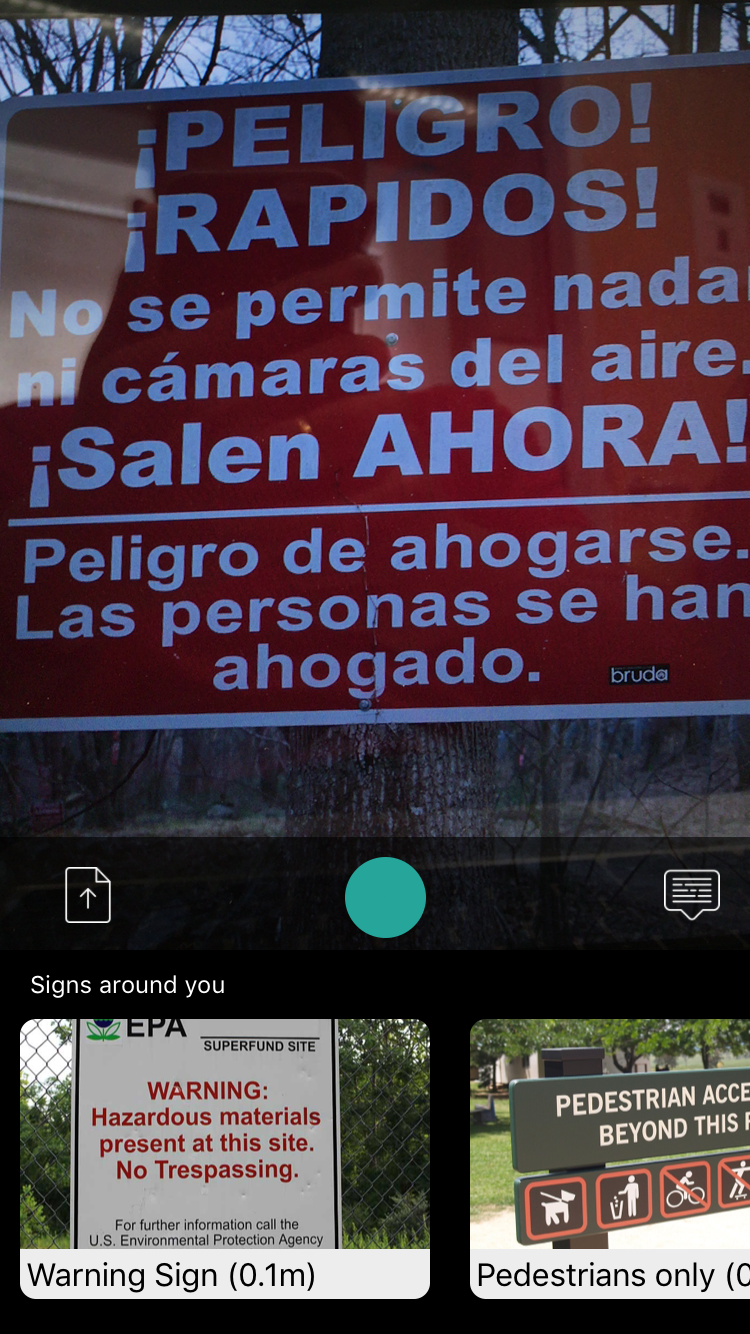
\includegraphics[width=0.5\linewidth]{media/1a.PNG}
	\caption{Affordance design principle}
	\label{fig:affordance}{This is the concept in which the physical characteristics of an object influence it's function. We have clearly separate individual functions using primary colors and appropriate icons. The main features of the application is loaded by default without the user having to make any clicks or taps.}
\end{figure} 

    
    
     \subsubsection{Visibility}
     \paragraph{}The usability is improved when its status and methods of how to use are clearly visible, intuitively. The more visible functions are, the more likely users will be able to understand how the system works \cite{norman}. In contrast, when functions are 'out of sight,' it makes them more difficult to find and understand the application.
     
         \paragraph{} In the mobile application developed, the capture picture button has a green color, so as to invite the user to click the button. The camera functionality also has an 'upload image' icon and 'type and translate' icon present upfront. Their is no ambiguity in the user interface. The digital signage section also lists the nearby digital signages along with the title and distance from the user. This improves the visibility of all the features of the app without the user having to scroll down. 
     
      \subsubsection{Constraint} 
      
      \paragraph{}The design concept of constraining refers to determining ways of restricting the kind of user interaction that can take place at a given moment \cite{norman}. This helps the application to do what it is exactly supposed to do and eliminates many error scenarios. This is helpful for the stable functioning of the application.
      
      \paragraph{}In the system we built, we establish constraints by only listing the digital signages around. If there are no digital signages around, 'No digital signages around' message is shown to the user. Also, the system is constrained to capture/upload only one image and use web-services to extract text from it. This helps the application function without many errors. 
      
      
      
       \subsubsection{Consistency}
       \paragraph{}This refers to designing interfaces to have similar operations and use similar elements for achieving similar tasks \cite{norman}. In particular, a consistent interface is one that follows rules, such as using the same operation to select all objects. This helps the user intuitively learn and use the application without having to spend more time on it \cite{norman}. 
       
       \paragraph{}In our study, we have designed the UI using the modules approach. That is, whether the user chooses to capture an image or upload from the camera roll, the layout is the same. In the digital signages section, all the signages are listed consistently and the whole thumbnail is clickable. Each click takes the user to a screen with more details about the signage. This page is designed consistently. This helps the user to understand our application faster.
       
        \subsubsection{Feedback}
       \paragraph{}Feedback is about informing the user about what action has been done and what has been accomplished, allowing the user to continue with the activity \cite{norman}. This helps the user to understand there is a background process running and at the same time, the user is constrained from starting another process or quitting the current process. 
       
       \paragraph{}In the application developed, the user is shown 'loading' icon when a background process is running, for example, when an image is being uploaded through web-services. This helps the user understand that there is a process running in the background and also helps the user to understand the application better. Also, appropriate error messages are shown at the appropriate places to help user understand about the action being carried out \cite{norman}.
       
       \begin{figure}[H]
	\centering
	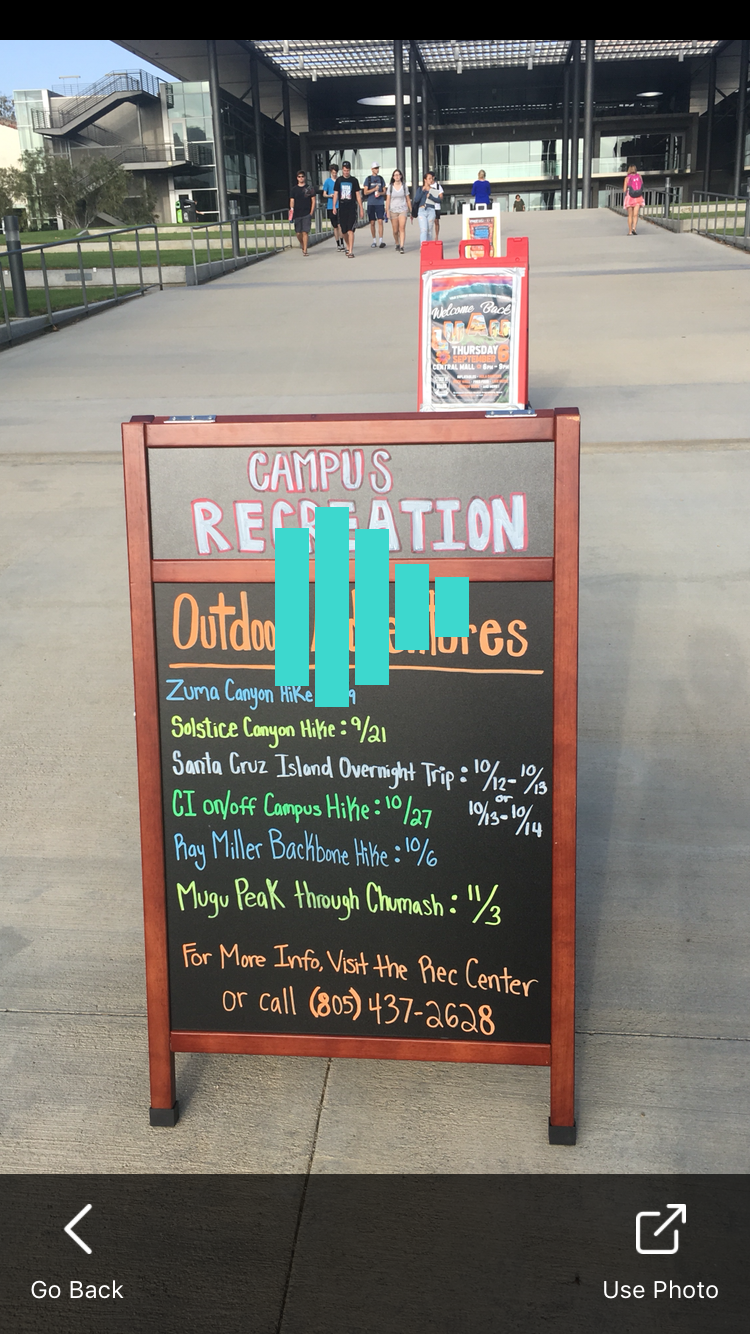
\includegraphics[width=0.5\linewidth]{media/loading1.PNG}
	\caption{Feedback design principle}{We added a 'loading' animation to let the user know that there is a process running on the background.}
	\label{fig:feedback}
\end{figure} 

%Case study
\section{Case study}
\label{evaluation}

%\paragraph{}As an evaluation experiment of this system, the multilingual digital signage constructed in this study was placed in the library of the university campus, and the students, including foreign students were handed out smartphones running the mobile application and were asked to use the multilingual digital signage system.
%
%\paragraph{}For evaluation, different signages with information from the library office was displayed in Spanish language. After the use of the system, 20 students that include 10 American students and 10 international/foreign students were asked to answer a questionnaire and an interview. This is to simulate the 'foreign-visitor' environment. This is important for our study because foreign visitors are our primary users.


\paragraph{}We conducted a small scale evaluation of the multilingual digital signage system as mentioned in Section \ref{system}. The purpose of this evaluation is to study the feasibility of using the inexpensive iBeacons along with computer vision features of the system. We set up a combination of digital and printed signages in a room. We set up three iBeacons along with two printed signages and measuring points in a room, approximately 45m x 35m.

\paragraph{}The iBeacons used in this experiment were Gimbal Series 10 beacons, distributed by Gimbal. For reception, we used installed the developed mobile application on iPhone 6s, running iOS version 11.3. We also setup two printed signages with information in Spanish language and placed them around the library, at least 30 meters apart.

\subsection{Testing environment}

\paragraph{}Three iBeacons were configured as digital signages and setup along
with two printed signages in a room, approximately 45m x 35m. The developed mobile application was installed on iPhone 6s, running iOS version 11.3 with a 4G network. Table \ref{my-test} shows the testing environment for case study.

\begin{table}%[H]
    \centering
    
    \label{my-test}
       \begin{tabular}{|p{30mm}|p{55mm}|p{35mm}|}
 \hline
  & \textbf{Data}  \\ [0.5ex] 
 \hline\hline
 \textbf{Smartphone} & iPhone 6s \\
 \hline
  \textbf {iOS version} & 11.3 \\
 \hline
 \textbf{Internet} & LTE  and Wi-Fi \\
 \hline
 \textbf{iBeacons} & Gimbal  Series 10  \\
 \hline
 
    \end{tabular}
    \caption{Testing environment } 
\end{table}

\subsection{Digital Signages }

\paragraph{}These include the signages with iBeacons installed. There are two interactions during the discovery of nearby digital signages from the mobile application. The first part is interaction between iBeacons and the user. iBeacon will broadcast signals at a certain interval, if the smartphone detects and locates the iBeacons around it,  the application can handle the iBeacon event based on proximity location information, including major ID, minor ID and distance. The second part is interaction between the mobile application and database. During this interaction, the application should fetch respective information and display on the mobile application.

\subsubsection{Test Case 1}
\label{oneone}
\paragraph{}With the above mentioned setup of the signages inside the campus library, we use the mobile application to evaluate the feasibility of the proposed system. Each signage is at least 20 meters away from each other. We downloaded the developed mobile application on to the iPhone 6s and walked towards the room.

\paragraph{}The mobile application picked up the closest digital signage when the user was 17.4 meters away. As and when the user walked towards the signage, the distance decreased appropriately. The other digital signages were listed at the distance of 22.3 meters and 27 meters away. On tapping each thumbnail of signage from the application, it fetched and displayed relevant signage information from the database. We were also able to translate the signage description from English to Spanish and the translation was 100\% correct.

\begin{table}%[H]
    \centering
  
    \label{my-label}
       \begin{tabular}{|p{30mm}|p{55mm}|p{35mm}|}
 \hline
  & \textbf{Data}  \\ [0.5ex] 
 \hline\hline
 \textbf{Discovered} & 27.4 meters away  \\ 
 \hline
 \textbf{Fetched signage data} & "Hazardous materials present at this site. No trespassing."  \\
 \hline
 \textbf{Text translated} &  "Materiales peligrosos presentes en este sitio. Prohibido el paso. No hay vehículos más allá de este punto. Los vehículos autorizados deben exhibir permisos para ingresar. Zona bajo estricta vigilancia." \\
 \hline
 \textbf{Error in text translated} & 0\%   \\ [1ex] 
 \hline
    \end{tabular}
      \caption{Observations from test case 1}{We find that the digital signage was discovered 27.4 meters away from the user and the appropriate message is translated to Spanish with 0\% error} 
\end{table}


       \begin{figure}[H]
	\centering
	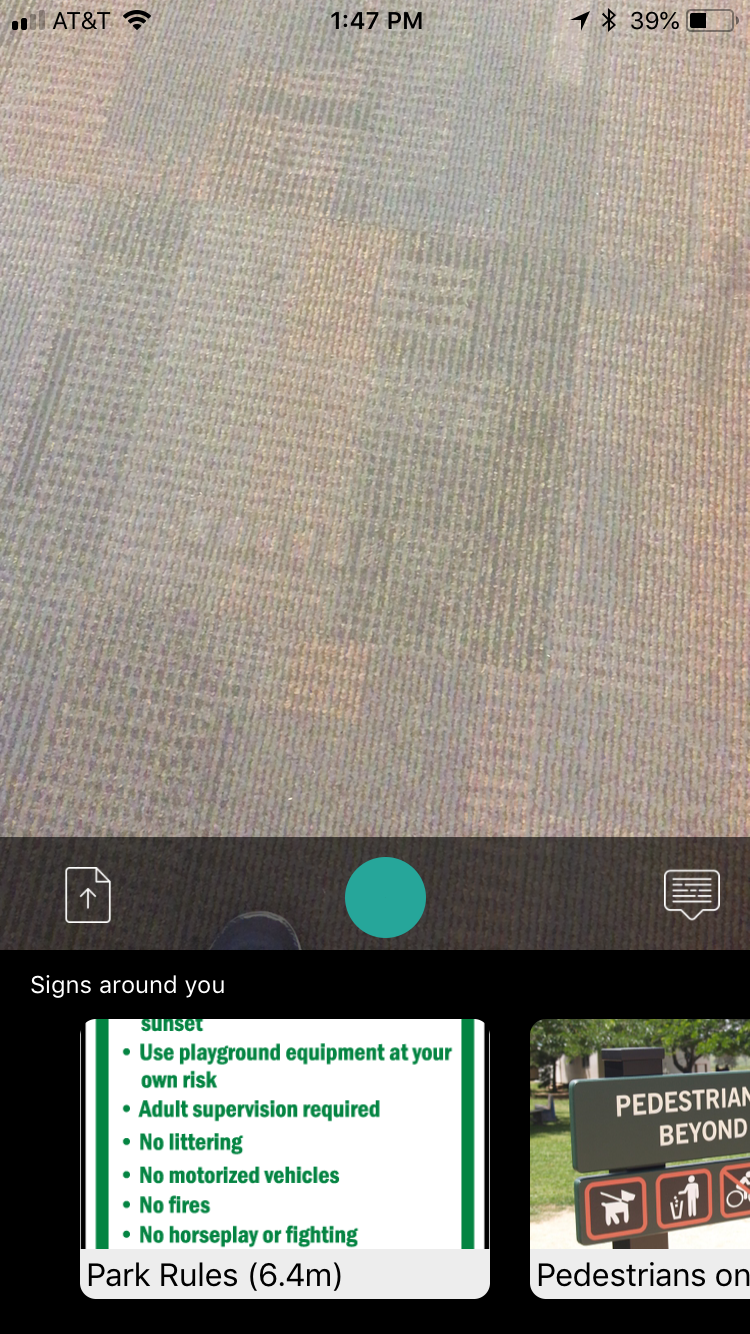
\includegraphics[width=0.5\linewidth]{media/test1.png}
	\caption{Digital signage 1}{We notice that the digital signage called 'Park Rules' is discovered form the mobile application at a distance of 6.4 meters away}
	\label{fig:engyo}
\end{figure} 

%Test case 2
\subsubsection{Test Case 2}
\label{one2one}
\paragraph{}For this test case, we setup the digital signages closer than the previous test case. The aim of this test case is to evaluate for interference in beacon signals. Each signage was installed  15 meters away from each other. We ran the developed mobile application on the iPhone 6s and walked towards the room.

\paragraph{}The mobile application picked up the closest digital signage when the user was 23.4 meters away. The other digital signages were listed at the distance of 26.3 meters and 35.7 meters away. On tapping each thumbnail of signage from the application, it fetched and displayed relevant signage information from the database. We were also able to translate the signage description from English to Spanish and the translation was 100\% correct.

\paragraph{}This proves that the digital signage system can be set up in close proximity to each other and the system will not face any interference from the crowded iBeacon signals. 

       \begin{figure}[H]
	\centering
	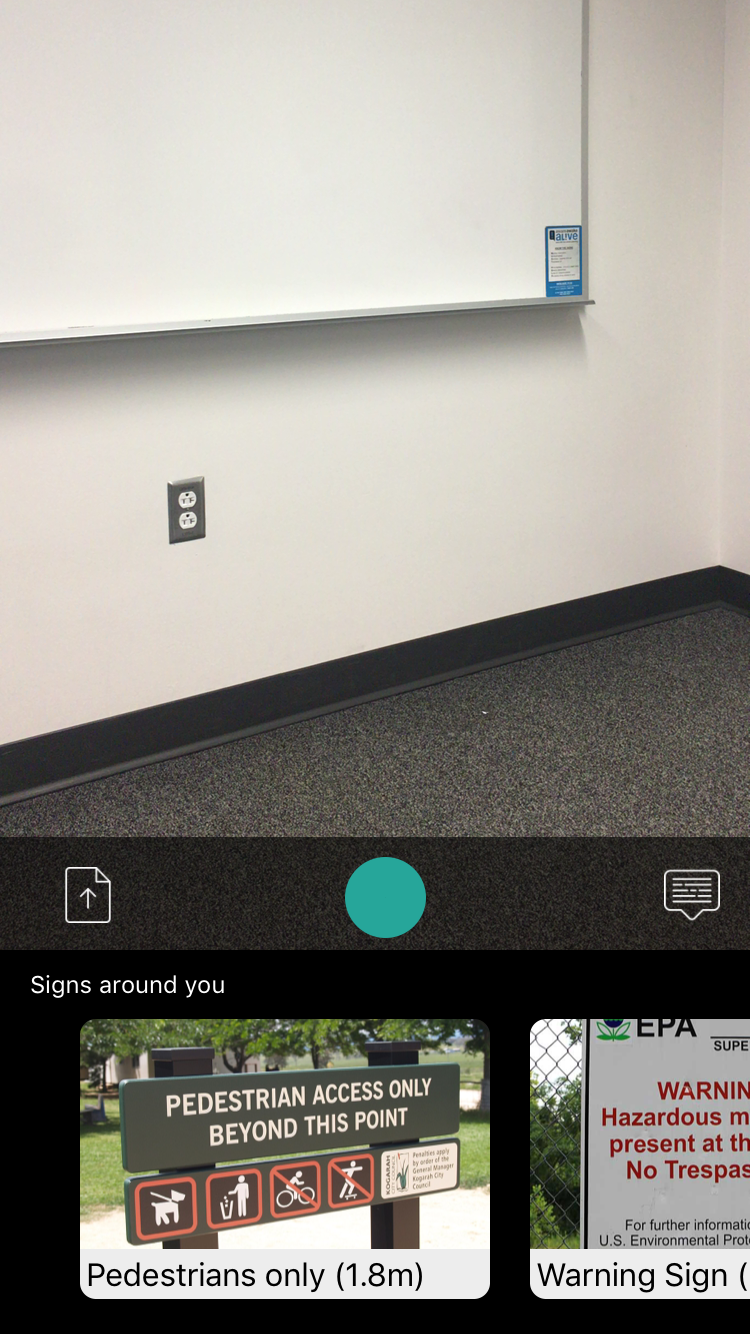
\includegraphics[width=0.5\linewidth]{media/case1.png}
	\caption{Digital signage 2} {When the digital signages are placed in close proximity to each other, the mobile application does not interfere with the crowded signals. Hence, the mobile application works when we setup the signages in close proximity.}
	\label{fig:eng}
\end{figure} 

\begin{table}%[H]
    \centering
   
    \label{my-label}
       \begin{tabular}{|p{30mm}|p{55mm}|p{35mm}|}
 \hline
  & \textbf{Data}  \\ [0.5ex] 
 \hline\hline
 \textbf{Discovered} & 19.4 meters away  \\ 
 \hline
 \textbf{Fetched signage data} & "Pedestrian access only beyond this point."  \\
 \hline
 \textbf{Text translated} &  "Acceso peatonal solo más allá de este punto." \\
 \hline
 \textbf{Error in text translated} & 0\%   \\ [1ex] 
 \hline
    \end{tabular}
     \caption{Observations from test case 2} {We notice that another printed signage was discovered at a distance of 19.4 meters away from the user. On tapping the thumbnail on the mobile application, the system fetched the relevant details of the signage. We could also translate the fetched information into Spanish with 0\% error.}
\end{table}


\subsection{Printed Signages }
\label{twoone}
\paragraph{}The other scenario we need to evaluate is the multilingual translation of printed signages (signages without iBeacons installed). When the user clicks an image of a signage, the mobile application should be able to extract text and translate it to the user's preferred language without missing critical information. We evaluate the feasibility of the system in the following scenarios.

\subsubsection{Test Case 3}
\label{threetwo}
\paragraph{}We use the same mobile application used in test cases 1 and 2 to evaluate the feasibility of the system to extract text and translate it from Spanish to English. We positioned the mobile application at a distance of 35 feet from the signage.

\paragraph{}To evaluate the text extraction and translation from printed signage, we clicked a picture of the printed signage. The application extracted relevant text from the printed signage. The application also supported the translation of the extracted text to Spanish language and the translation was 100\% correct.

\paragraph{}We noticed an 0\% error in the text extraction and text translation from Spanish to English. Below figures  \ref{fig:case3} and \ref{fig:eng} show the flow of the text extraction and translation for printed signage 1.


 \begin{figure} [H]
\centering
\begin{minipage}{.5\textwidth}
  \centering
  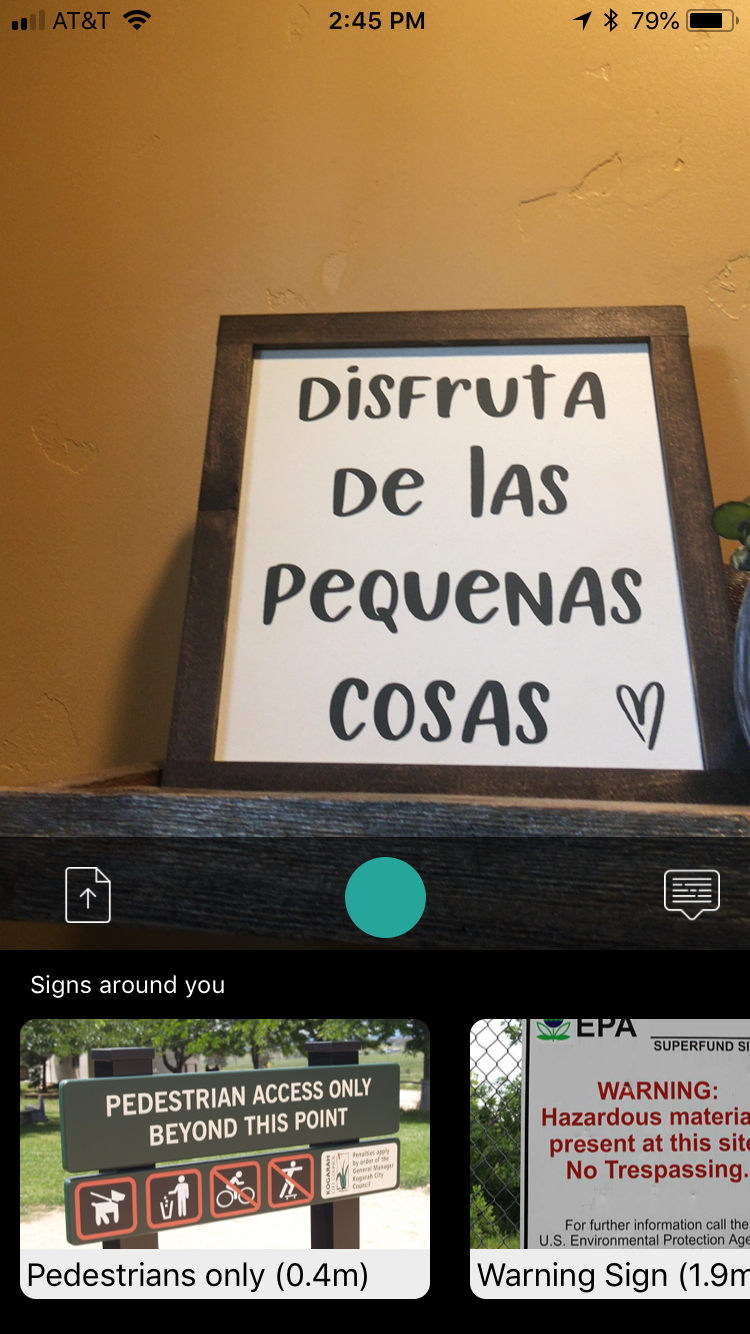
\includegraphics[width=0.9\linewidth]{media/1.png}
  \caption{Printed Signage 1}{The screenshot shows the mobile application about to capture the image of a printed signage in Spanish language.}
  \label{fig:case3ins}
\end{minipage}%
\begin{minipage}{.5\textwidth}
  \centering
  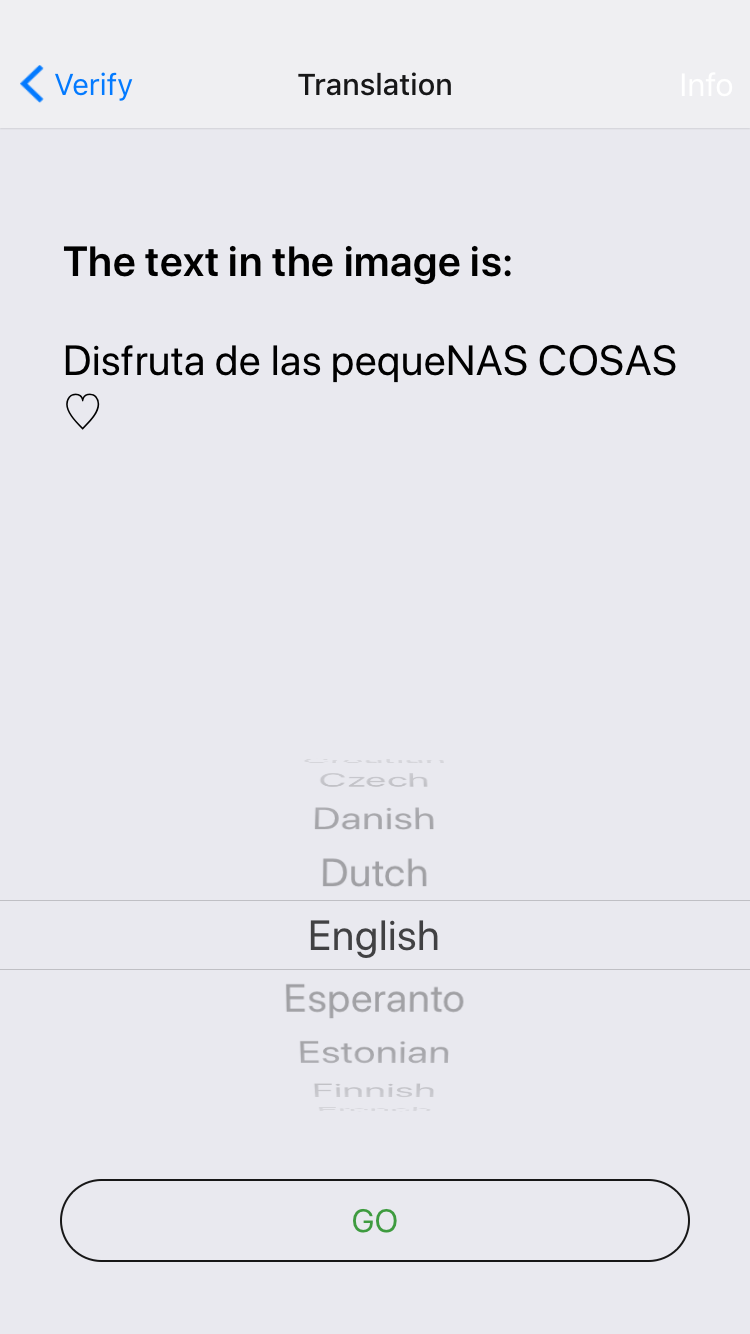
\includegraphics[width=0.9\linewidth]{media/case3.PNG}
  \caption{OCR feature}{This screenshot shows the text extracted from the printed signage shown in Figure \ref{fig:case3ins}. We used OCR feature to extract the text.}
  \label{fig:case3}
\end{minipage}
\end{figure}

       \begin{figure}[H]
	\centering
	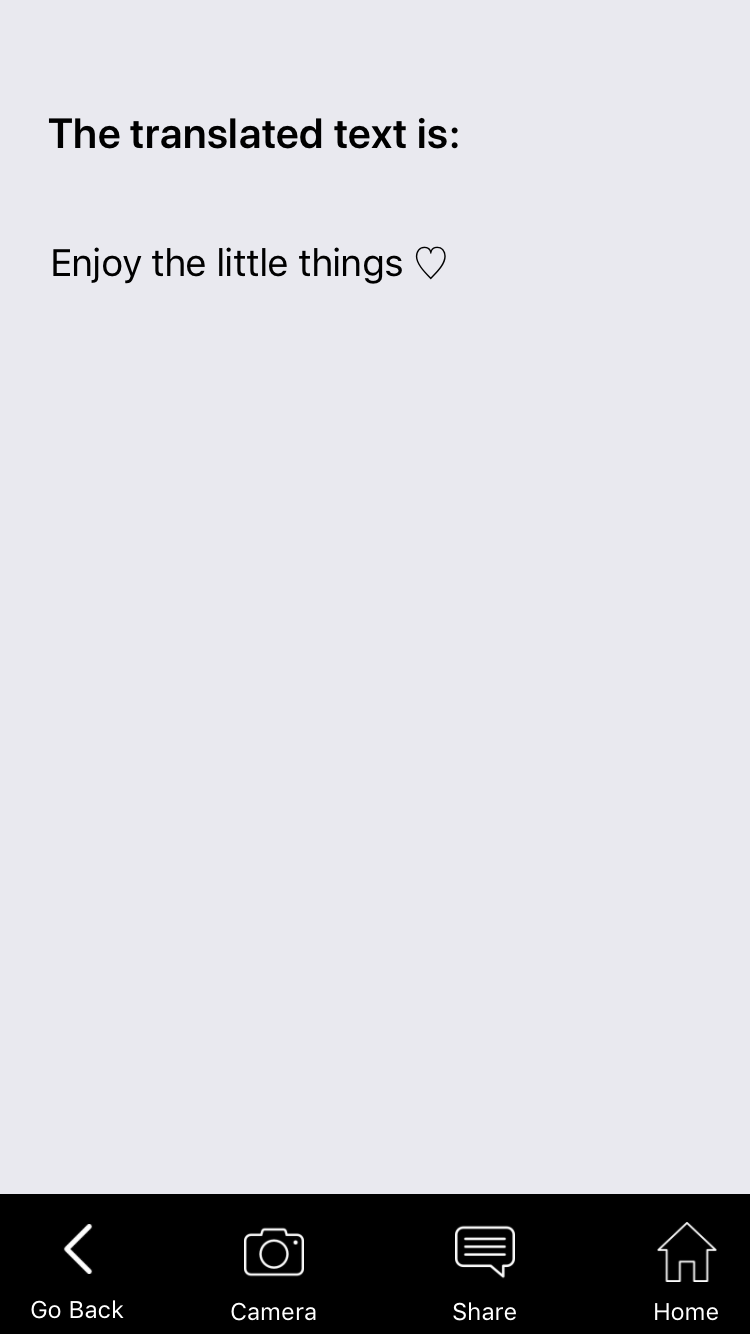
\includegraphics[width=0.5\linewidth]{media/case3-eng.PNG}
	\caption{Text translated to English}{The extracted text from figure \ref{fig:case3ins} is then translated to English using the Google Translate API. We notice that the text is translated with 0\% error, including the emoticon. }
	\label{fig:eng}
\end{figure} 


\begin{table}%[H]
    \centering
   
    \label{my-label3}
       \begin{tabular}{|p{30mm}|p{55mm}|p{35mm}|}
 \hline
  & \textbf{Data}  \\ [0.5ex] 
 \hline\hline
 \textbf{Image captured from} & iPhone 6s  \\
 \hline
  \textbf{Text extracted} & "Disfruta de las pequenas" \\
 \hline
 \textbf{Text translated} & "Enjoy the little things"   \\
 \hline
 \textbf{Error in text extraction} & 0\%   \\
 \hline
 \textbf{Error in text translated} & 0\%   \\ [1ex] 
 \hline
    \end{tabular}
     \caption{Observations from test case 3} {The table shows the text extracted from the printed signage shown in Figure  \ref{fig:case3ins}. We notice that the text is extracted from the Spanish printed signage and translated to English with 0\% error in text extraction and translation}
\end{table}

\subsubsection{Test Case 4}
\label{threefour}
\paragraph{}For this test case, we use another printed signage with information in Spanish language and use our system to extract the text and translate it to English. The aim of this test case is to evaluate the text extraction and translation of different languages. 

\paragraph{}To evaluate the text extraction and translation from a Spanish printed signage, we clicked a picture of the printed signage. The application extracted relevant text from the printed signage. The application also supported the translation of the extracted Spanish text to English language and the translation was 91\% correct.

\paragraph{}We noticed an 8\% error in the text extraction feature and thereby the same error while translating the text to English. Below Figure \ref{fig:case4in}, \ref{fig:case4} and \ref{fig:engs} show the flow of the text extraction and translation for signage 2.

 \begin{figure} [H]
\centering
\begin{minipage}{.5\textwidth}
  \centering
  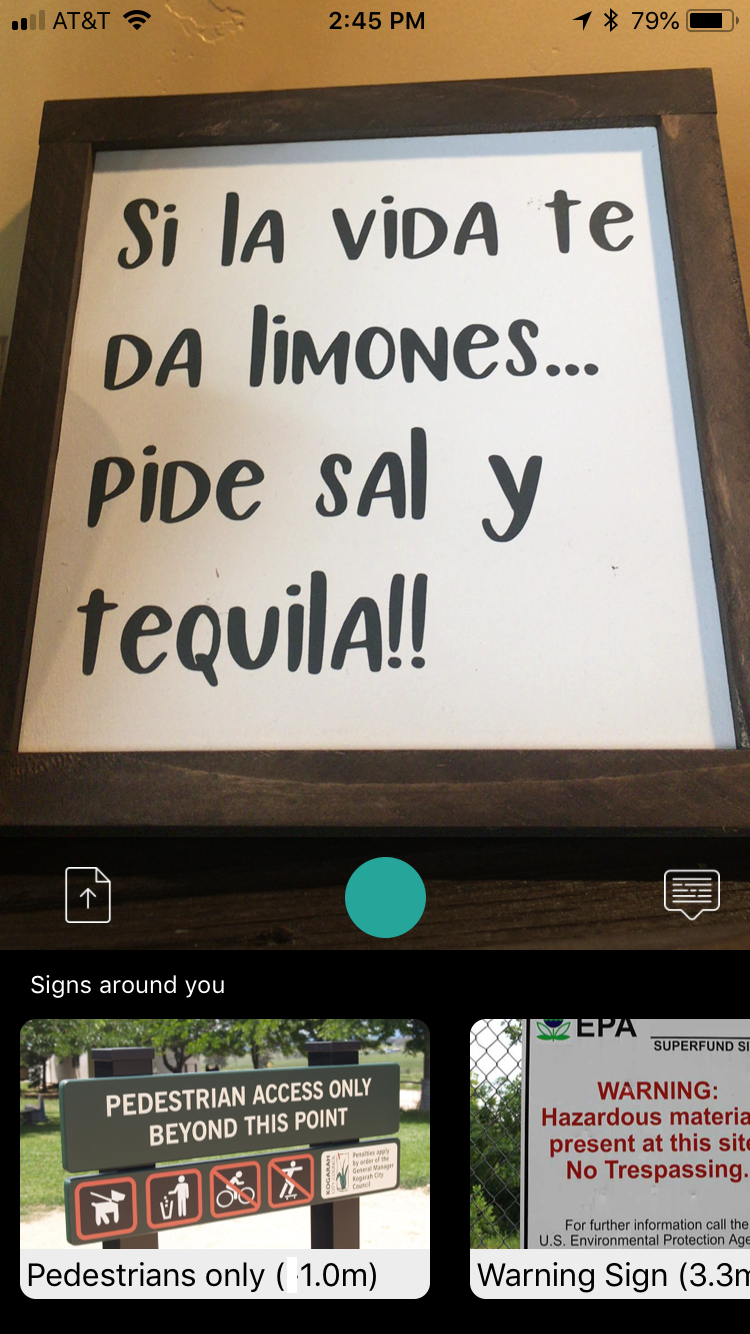
\includegraphics[width=0.9\linewidth]{media/case4.png}
  \caption{Printed Signage 2}{The screenshot shows the mobile application about to capture the image of a printed signage in Spanish language}
  \label{fig:case4in}
\end{minipage}%
\begin{minipage}{.5\textwidth}
  \centering
  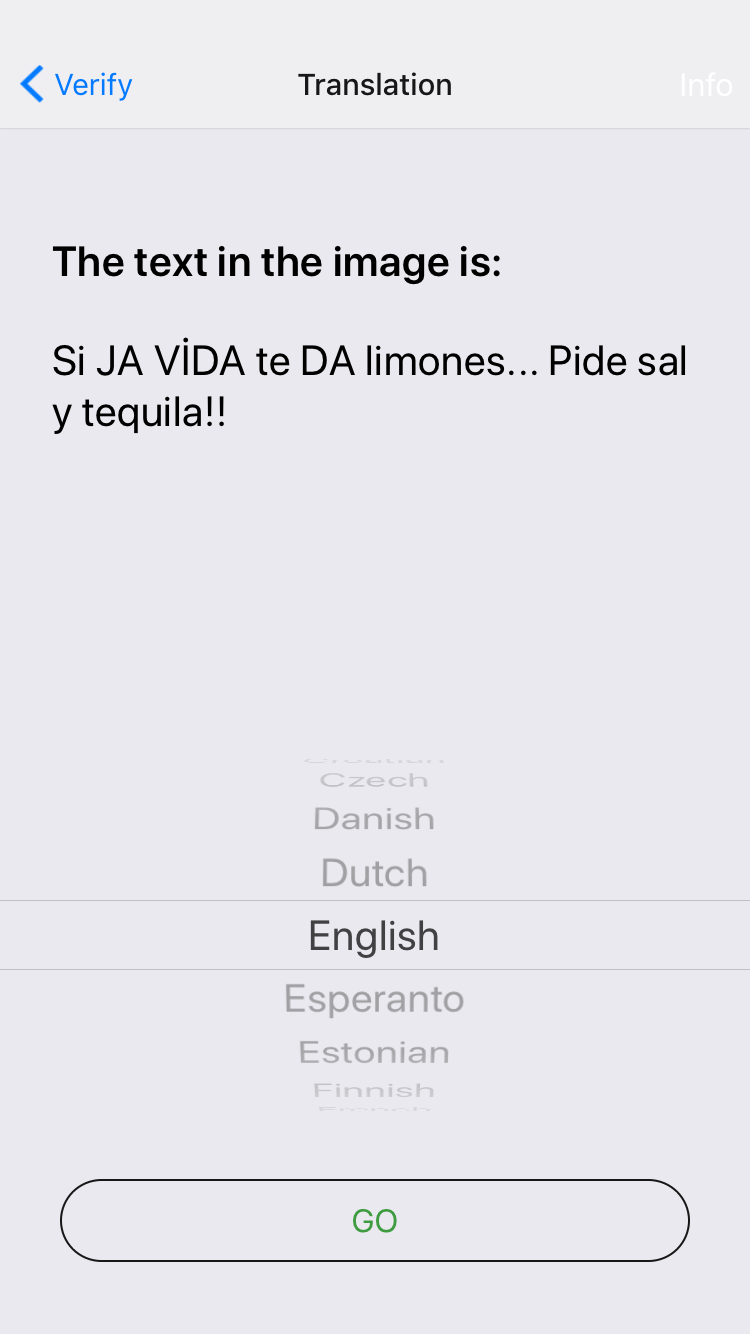
\includegraphics[width=0.9\linewidth]{media/case4a.png}
  \caption{OCR feature}{This screenshot shows the text extracted from the printed signage shown in Figure \ref{fig:case4in}. We used OCR feature to extract the text.}
  \label{fig:case4}
\end{minipage}
\end{figure}

       \begin{figure}[H]
	\centering
	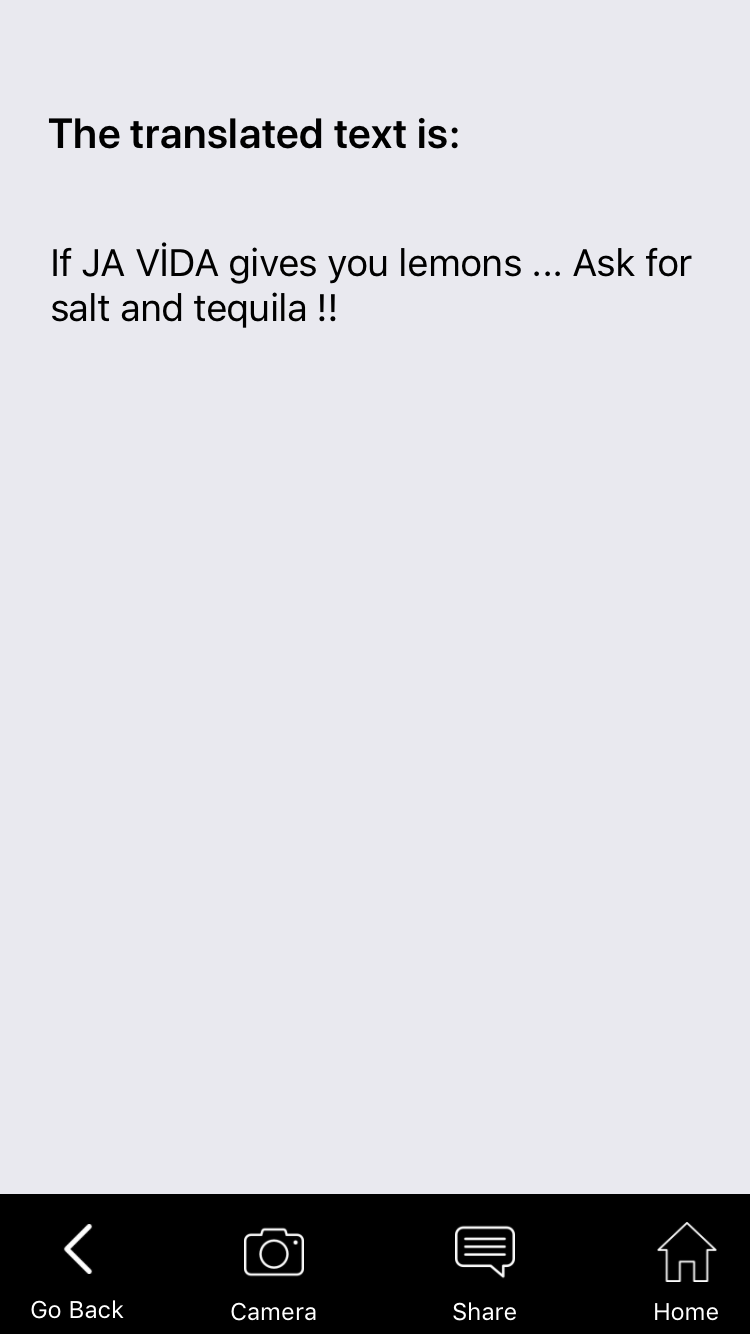
\includegraphics[width=0.5\linewidth]{media/case4b.png}
	\caption{Text translated to English}{The extracted text from Figure \ref{fig:case4in} is then translated to English using the Google Translate API. We notice that the text is extracted with with 4\% error and 8\% error in text translation.}
	\label{fig:engs}
\end{figure} 

\begin{table}%[H]
    \centering
   
    \label{my-label4}
       \begin{tabular}{|p{30mm}|p{55mm}|p{35mm}|}
 \hline
  & \textbf{Data}  \\ [0.5ex] 
 \hline\hline
 \textbf{Image captured from} & iPhone 6s \\
 \hline
  \textbf{Text extracted} & "Si la vida te Da limonoes... pide sal y tequila!!"  \\
 \hline
 \textbf{Text translated} & "If JA VIDA gives you lemons... Ask for salt and tequila !!"   \\
 \hline
 \textbf{Error in text extraction} & 4\%   \\
 \hline
 \textbf{Error in text translated} & 8\%   \\ [1ex] 
 \hline
    \end{tabular}
     \caption{Observations from test case 4} {The table shows the text extracted from the printed signage shown in Figure 19. We notice that the text is extracted from Spanish language with with 4\% error and 8\% error in text translation from Spanish to English language.}
\end{table}

%\subsection{Questionnaire}
%
%\paragraph{}We developed the below questionnaire to evaluate the system. The subjects were asked to answer the questions using the five grade system. 
%
%\paragraph{}1. Have you faced the problems of not understanding signages when visiting foreign countries?
%\begin{itemize}
%	\item Strongly agree
%	\item Agree
%	\item Neither agree or disagree
%	\item Disagree
%	\item Strongly disagree
%\end{itemize}
%
%\paragraph{}
%
%\paragraph{}2. Do you think this system solves the language problem?
%\begin{itemize}
%	\item Strongly agree
%	\item Agree
%	\item Neither agree or disagree
%	\item Disagree
%	\item Strongly disagree
%\end{itemize}
%\paragraph{}
%
%\paragraph{}3. Do you feel the application is easy to use?
%\begin{itemize}
%	\item Strongly agree
%	\item Agree
%	\item Neither agree or disagree
%	\item Disagree
%	\item Strongly disagree
%\end{itemize}
%\paragraph{}
%
%\paragraph{}4. Would you like to use this application in the future?
%\begin{itemize}
%	\item Strongly agree
%	\item Agree
%	\item Neither agree or disagree
%	\item Disagree
%	\item Strongly disagree
%\end{itemize}
%
%\paragraph{}
%\paragraph{}5. Would you recommend this application to your friends?
%\begin{itemize}
%	\item Strongly agree
%	\item Agree
%	\item Neither agree or disagree
%	\item Disagree
%	\item Strongly disagree
%\end{itemize}
%
%\paragraph{} Question 1 asks the subjects if they have faced any problems in understanding the signages when visiting foreign countries. This helps us understand if there is a definite need of a multilingual signage system. Question 2 asks if the introduced system helps in solving the linguistic problem. This helps us understand if our system solves the problem.
%
%\paragraph{}Questions 3 and 4 are targeted towards understanding the usability aspect of the system. This helps us make sure the design and user-experience of the system is effective and the 'usability'  goals are met. 
%
%\paragraph{}Question 5 asks the subjects if they would recommend this system to their friends and family. This helps us understand what the user concretely feels about the system.
%
%\subsection{Survey Results}
%
%\textbf{Insert Pie chart here}
%
%\paragraph{}From the results, the percentages of the answers of “strongly agree” and “agree” were 90\% in Questions 1 and 2. 90\% of the subjects had faced problems with reading signages in foreign countries. Also, 90\% of them believe this system can solve the problem.
%




\section{ Conclusion and future work}
\label{sect-conclusion}
\paragraph{}We studied the feasibility of using the combination of inexpensive iBeacons and computer vision to construct a system of multilingual digital signages. We conducted a preliminary experiment using an actual room to estimate the positioning accuracy and accuracy of language translation. When three beacons, placed on individual signages, we were able to discover them from the mobile application when in proximity. We were able to fetch respective data from the server and display signage information on the mobile application. We could also translate the information to any of the supported languages. Using the same mobile application, we could also extract text from printed signages and translate the same into different languages with acceptable context of translation. We believe this level of accuracy is acceptable for a system of multilingual digital signage. This system proves to be useful for non-native visitors to understand their surroundings better and obtain critical information using the mobile application. 

%\paragraph{} 
%
%\begin{itemize}
%	\item Evaluation experiment proves that the system is helpful to understand all kinds of signages in foreign countries. 
%	\item The construction of low-cost digital signage system proves to be effective in understanding the signages better for a foreign visitor
%	\item The usability goals of the mobile application and the system as a whole is met.
%\end{itemize}

% \paragraph{}The system in study could be scaled to be installed in any physical 

\paragraph{}Future work could be done on determining user's position in the network of iBeacons by triangulating the user's position using the RSSI of three beacons in the network . Further, the user experience of the mobile application could be enhanced by translating just the text in the signage while maintaining the graphics like color and font of the signage. The system in this research could also be extended to be used in museums and shopping malls.

%
%\begin{itemize}
%	\item Determining the user's position in a network of beacon, thereby implementing indoor navigation.
%	\item Translating the whole signage, while maintaining the format and graphics of the signage. 
%\end{itemize}


\cleardoublepage
\phantomsection
%\bibliographystyle{plain}
\bibliographystyle{ieeetr}
\bibliography{references}
\addcontentsline{toc}{section}{References}

\end{document}

